% Kapitel 4 – wird von masterarbeit.tex / abgabe.tex eingebunden
\chapter{Experimente und Ergebnisse}
\label{ch:results}

Dieses Kapitel beschreibt die Experimente auf dem Datensatz GazeCapture
\cite{krafka2016itracker} und auf meinen eigenen Aufnahmen. Zuerst erkläre ich
Modell, Daten und Auswertung (\cref{sec:setup}). Danach folgen die
Trainingseinstellungen (\cref{sec:training}), die räumliche Verteilung des
Fehlers und die Loss Functions (\cref{sec:spatial}) und schließlich die
Personalisierung (\cref{sec:sessions,sec:loading,sec:session_design}).
\Cref{sec:discussion} fasst zusammen, was die Ergebnisse bedeuten.

Alle Zahlen wurden mit den Protokolldateien der Experimente abgeglichen. Dabei
wurde ein Fehler im Auswertungscode gefunden und korrigiert (\cref{sec:metric}).
Alle Werte in den Tabellen verwenden die korrigierte Metrik. Die Lernkurven in
\cref{fig:normalization} (unten) und \cref{fig:lr_curves} stammen dagegen aus
älteren Einzelläufen mit einer anderen Datenauswahl; die Bildunterschriften
nennen die Unterschiede.

% ==============================================================================
\section{Versuchsaufbau}
\label{sec:setup}
% ==============================================================================

Modell, Training, Daten und Auswertung sind in \crefoder{ch:methodik}{Kapitel~3 der
Masterarbeit} beschrieben. Hier stehen nur die Details, die man für die
Experimente zusätzlich braucht. Die Standardwerte zeigt
\cref{tab:default_config}.

\subsection{Daten und Splits}
\label{sec:data}

Die verwendete Teilmenge von GazeCapture und die beiden Splits
\code{norm\_subject} und \code{norm\_random} sind in
\crefoder{sec:meth_daten}{Kapitel~3 der Masterarbeit} beschrieben. Bei \code{norm\_random} liegen alle Bilder einer Person zum
selben Zielpunkt zusammen im Training oder im Test. Für die Hyperparameterstudie ziehe ich \num{1000} Trainings- und \num{200}
Testbilder \emph{zufällig} aus den Split-Dateien (fester Seed 0,
\code{--sample-seed 0}). Bei \code{norm\_subject} kommen die Trainingsbilder
von 179 Personen und die Testbilder von 45 anderen Personen. Ältere Läufe
haben einfach die \emph{ersten} Zeilen der sortierten Dateien genommen. Das
waren nur fünf Trainingspersonen und eine Testperson. Diese Läufe verwende ich
nicht mehr.

\subsection{Fehlermaß}
\label{sec:metric}

Alle Blickziele liegen im Einheitsquadrat $[0,1]^2$ (\cref{sec:normalization}).
Der Fehler ist die Wurzel aus dem mittleren quadrierten \emph{euklidischen}
Abstand zwischen Vorhersage $\hat{\bm p}_i$ und Ziel $\bm p_i$. Ich gebe ihn in
Prozent der Bildschirmdiagonale $\sqrt{2}$ an:
\begin{equation}
  \Ediag \;=\; 100\cdot
  \frac{\sqrt{\frac{1}{N}\sum_{i=1}^{N}\lVert\hat{\bm p}_i-\bm p_i\rVert_2^{2}}}{\sqrt{2}}
  \quad[\%].
  \label{eq:ediag}
\end{equation}
\SI{0}{\percent} bedeutet eine perfekte Vorhersage, \SI{100}{\percent} einen
Fehler so groß wie die ganze Bildschirmdiagonale.

\subsection{Ablauf der Experimente}
\label{sec:protocol}

Die Hyperparameterstudie startet mit dem Befehl
\begin{center}
  \code{python exp.py --experiment all --sample-seed 0 --val-size 200}
\end{center}
Ich ändere immer nur einen Wert (zum Beispiel die Batch Size). Alle anderen
Werte bleiben auf der Standardeinstellung (\cref{tab:default_config}). Jede
Einstellung wird fünfmal trainiert. Das Early Stopping nutzt eine eigene
Validierungsmenge von 200 Bildern einer weiteren Person. Ich gebe den
\emph{Test}fehler in der Epoch mit dem kleinsten Validierungsfehler an. Die
Testdaten werden also nie für die Modellauswahl benutzt. Die Tabellen zeigen
den mittleren Testfehler, das zweiseitige \SI{98}{\percent}-Confidence Interval
(CI) des Mittelwerts (Student-$t$, vier Freiheitsgrade) und die mittlere
Laufzeit.

\paragraph{Was die \enquote{Laufzeit} misst.} Die Laufzeit ist die echte
Dauer (Wall-Clock) \emph{eines ganzen Trainingslaufs}, gemittelt über die fünf
Läufe. Ein Lauf beginnt mit der Auswertung des untrainierten Modells
(Epoch~0) und endet, wenn das Early Stopping abbricht. Er enthält alle
Epochs und nach jeder Epoch die Auswertung auf Trainings-, Validierungs- und
Testdaten. Die Laufzeit ist \emph{nicht} die Zeit pro Epoch. Sie enthält
\emph{nicht} das Laden der Bilder und nicht die einmalige Berechnung der
Backbone-Features vor dem Lauf. Weil das Early Stopping verschieden früh
abbricht, zeigt die Zeit auch, wie lange sich eine Einstellung noch verbessert.

\begin{table}[htbp]
  \centering
  \caption[Standardeinstellung von \code{exp.py}]{Standardeinstellung von \code{exp.py}. Jede Variation ändert
           genau einen dieser Werte.}
  \label{tab:default_config}
  \small
  \begin{tabular}{ll@{\hspace{2.5em}}ll}
    \toprule
    Parameter & Wert & Parameter & Wert \\
    \midrule
    Split               & \code{norm\_subject} & Trainierbare Schichten & nur FC \\
    Trainings-/Testgröße & \num{1000} / \num{200}\textsuperscript{a} & Output Activation & Sigmoid \\
    Batch Size          & 32                   & Loss          & L1 (\code{standard}) \\
    Learning Rate            & $10^{-4}$            & Max.\ Epochs / Patience & 500 / 3 \\
    Weight Decay        & $10^{-5}$            & Validierungsmenge & 200 Bilder\textsuperscript{b} \\
    Wiederholungen      & 5                    & & \\
    \bottomrule
  \end{tabular}\\[1mm]
  \parbox{0.9\linewidth}{\footnotesize \textsuperscript{a}\,zufällig gezogen,
  Seed 0. \textsuperscript{b}\,von einer Person, die weder im Training noch im
  Test vorkommt.}
\end{table}

\paragraph{So liest man die Tabellen.} In jeder Hyperparametertabelle ist
die gewählte Option mit $\dagger$ markiert. Die Spalte \enquote{$p$ vs.\
$\dagger$} enthält den $p$-Wert eines zweiseitigen Mann-Whitney-$U$-Tests
zwischen den fünf Läufen dieser Option und den fünf Läufen der gewählten
Option. Ich verwende einen Rangtest, weil man mit fünf Läufen nicht prüfen
kann, ob die Werte normalverteilt sind, und weil einige Optionen einzelne
Ausreißer haben (zum Beispiel ein ReLU-Lauf mit \SI{46,98}{\percent}). Bei
$5+5$ Läufen ist der kleinste mögliche $p$-Wert $0,008$. Er bedeutet: \emph{jeder}
Lauf der einen Option ist besser als \emph{jeder} Lauf der anderen. Ein
Mittelwert ist nur dann \textbf{fett}, wenn die gewählte Option
\emph{signifikant besser} ist als jede andere Option der Tabelle ($p<0,05$ und
kleinerer Mittelwert).

Drei Punkte sind dabei wichtig:
\begin{enumerate}[nosep]
  \item \textbf{Gleiche Daten in allen Wiederholungen.} Der Seed legt
        Trainings-, Test- und Validierungsdaten fest. Die fünf Wiederholungen
        unterscheiden sich nur in den Startgewichten, der Reihenfolge der Daten
        und im Dropout. Das CI zeigt also die Zufälligkeit des Trainings, nicht
        den Einfluss anderer Datenteilmengen.
  \item \textbf{Kleine Validierungsmenge.} Die 200 Validierungsbilder stammen
        von nur einer Person. Das Early Stopping ist daher etwas zufällig. Die
        Testdaten werden aber nie für die Auswahl benutzt.
  \item \textbf{Trainingszeit.} Bei \enquote{nur FC} wird der Head auf
        gespeicherten ResNet-Features trainiert (512 Zahlen pro Bild statt
        des Bildes). Ein Lauf dauert daher nur etwa eine Sekunde, und
        Unterschiede in diesen Zeiten sind unwichtig. Bei FC + Layer~4 und beim
        vollen ResNet läuft in jeder Epoch jedes Bild vorwärts und rückwärts
        durch den Backbone. Diese Zeiten sind viel länger und nicht direkt mit
        \enquote{nur FC} vergleichbar.
\end{enumerate}

% ------------------------------------------------------------------------------
\subsection{Normierung der Zielwerte}
\label{sec:normalization}

Die rohen Blickziele in GazeCapture sind Bildschirmpunkte des jeweiligen
Geräts, gemessen von der oberen linken Ecke. Ihr Wertebereich hängt daher von
Bildschirmgröße und Ausrichtung ab. Die \num{347085} Bilder der 262 Personen
stammen von zehn Bildschirmformaten, von $320\times480$ bis $1024\times768$
Punkten, im Hoch- und im Querformat. Ich teile die Ziele deshalb durch die
Bildschirmbreite $W$ und -höhe $H$ des jeweiligen Bildes (\code{main.py}; Werte
außerhalb von $[0,1]$ werden abgeschnitten, das betrifft \SI{0,006}{\percent}
der Bilder):
\begin{equation}
  x_{\mathrm{norm}} = \frac{x}{W},\qquad y_{\mathrm{norm}} = \frac{y}{H}.
\end{equation}
\Cref{fig:normalization} zeigt die Wirkung. Ohne Normierung liegen die Ziele
der vielen Smartphone-Bilder vor allem oben links, und dieselbe Koordinate
bedeutet auf jedem Gerät eine andere Stelle (\cref{fig:raw_targets}). Die
Fehlerwerte sind dann zwischen Geräten nicht vergleichbar (linke Spalte). Nach
der Normierung liegen alle Ziele in $[0,1]^2$, und \cref{eq:ediag} ist sinnvoll
definiert (rechte Spalte). Alle weiteren Experimente verwenden normierte Ziele.

\begin{figure}[htbp]
  \centering
  \begin{subfigure}[t]{0.43\textwidth}
    \centering
    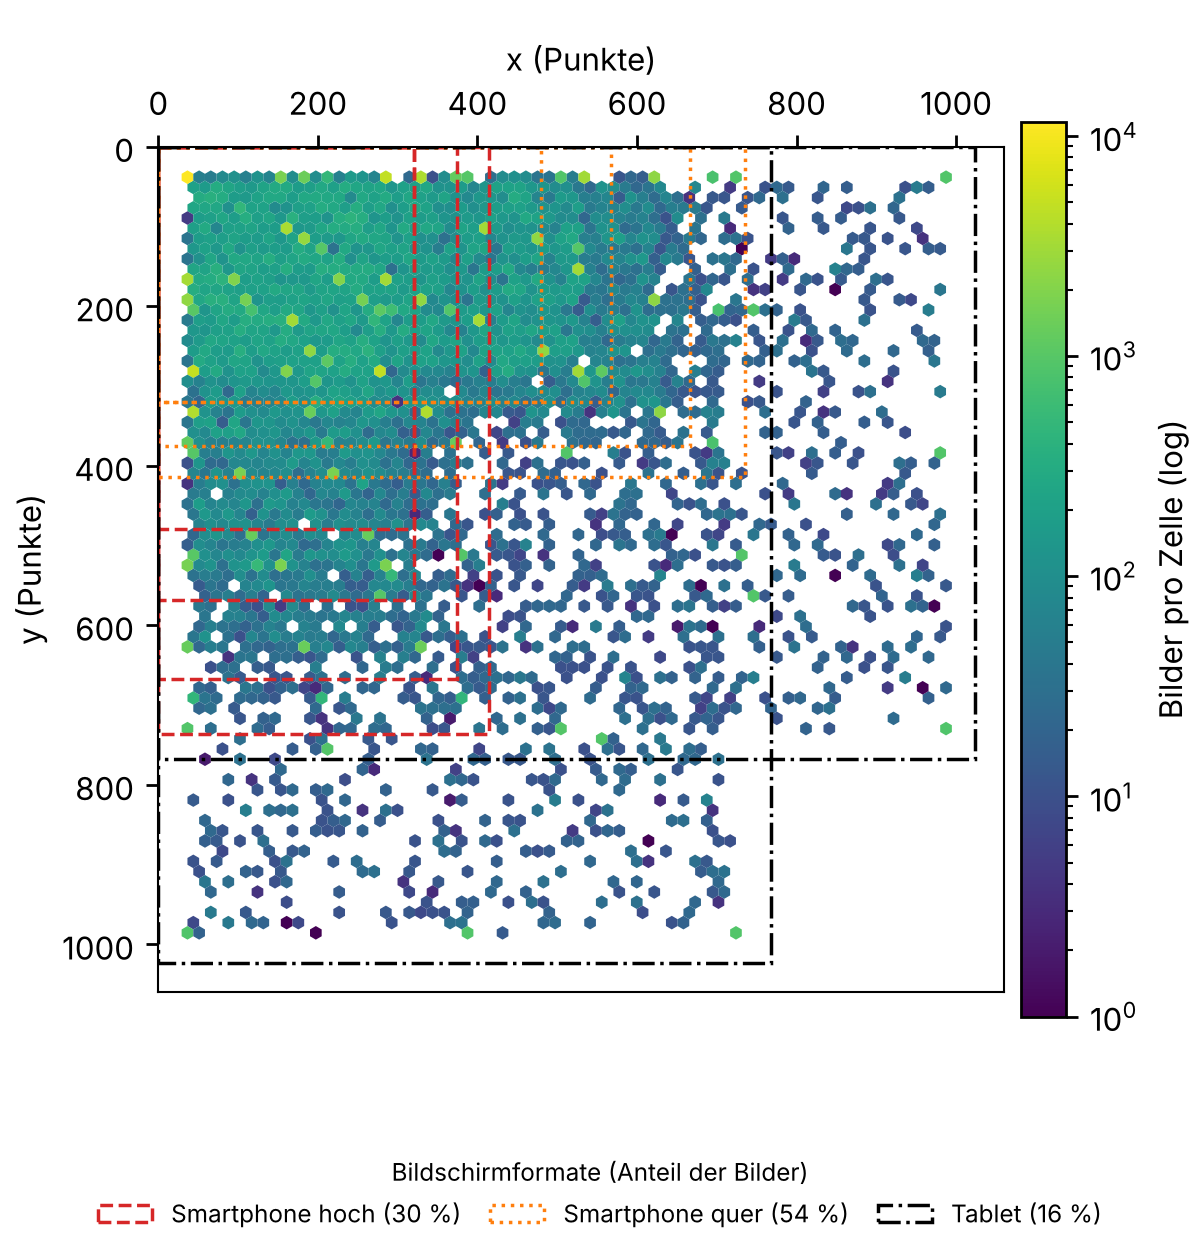
\includegraphics[width=\textwidth]{raw_targets.png}\\[2mm]
    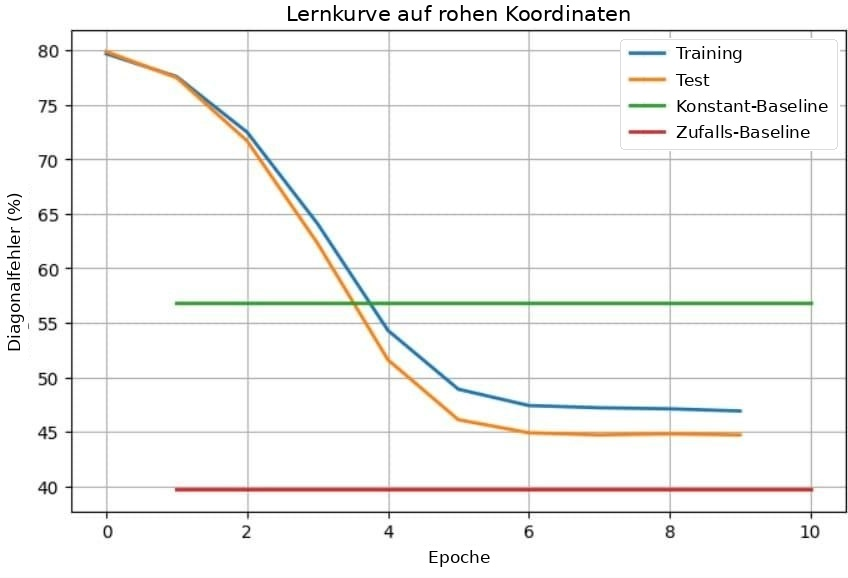
\includegraphics[width=\textwidth]{raw_learning_curve.png}
    \caption[Rohe Ziele in Bildschirmpunkten]{Rohe Ziele in Bildschirmpunkten (Dichte aller Bilder,
             logarithmische Farbskala); gestrichelt: Umrisse der
             Bildschirmformate. Unten: Lernkurve eines frühen Notebook-Laufs auf
             rohen Koordinaten; diese Werte sind keine Prozente einer
             gemeinsamen Diagonale und nicht mit den anderen Abbildungen und
             Tabellen vergleichbar.}
    \label{fig:raw_targets}
  \end{subfigure}
  \hfill
  \begin{subfigure}[t]{0.52\textwidth}
    \centering
    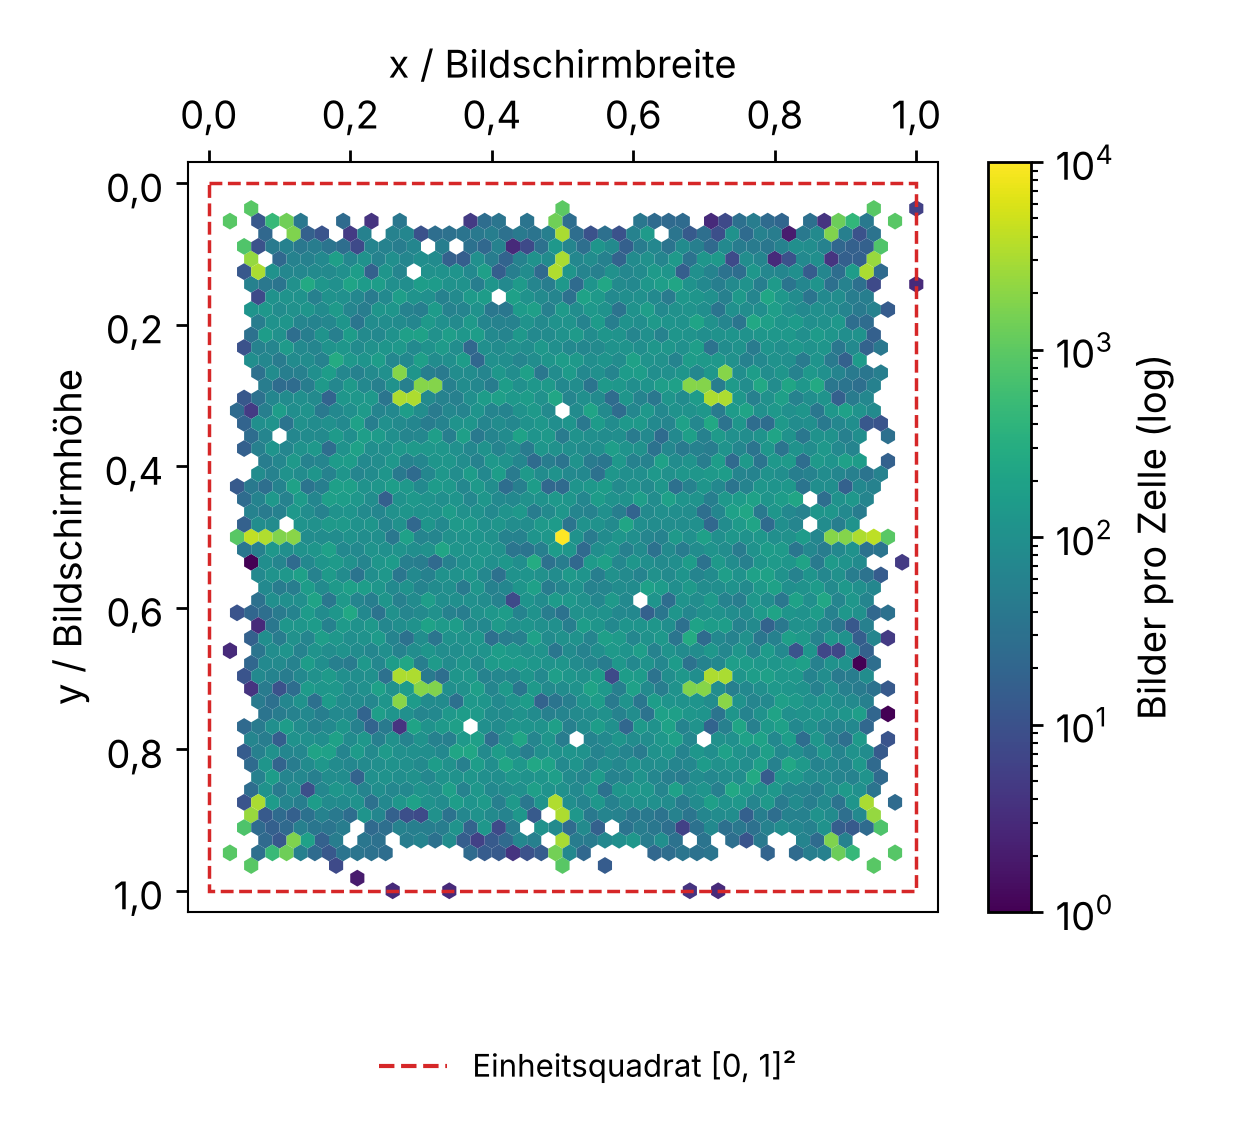
\includegraphics[width=0.82\textwidth]{normalized_targets.png}\\[2mm]
    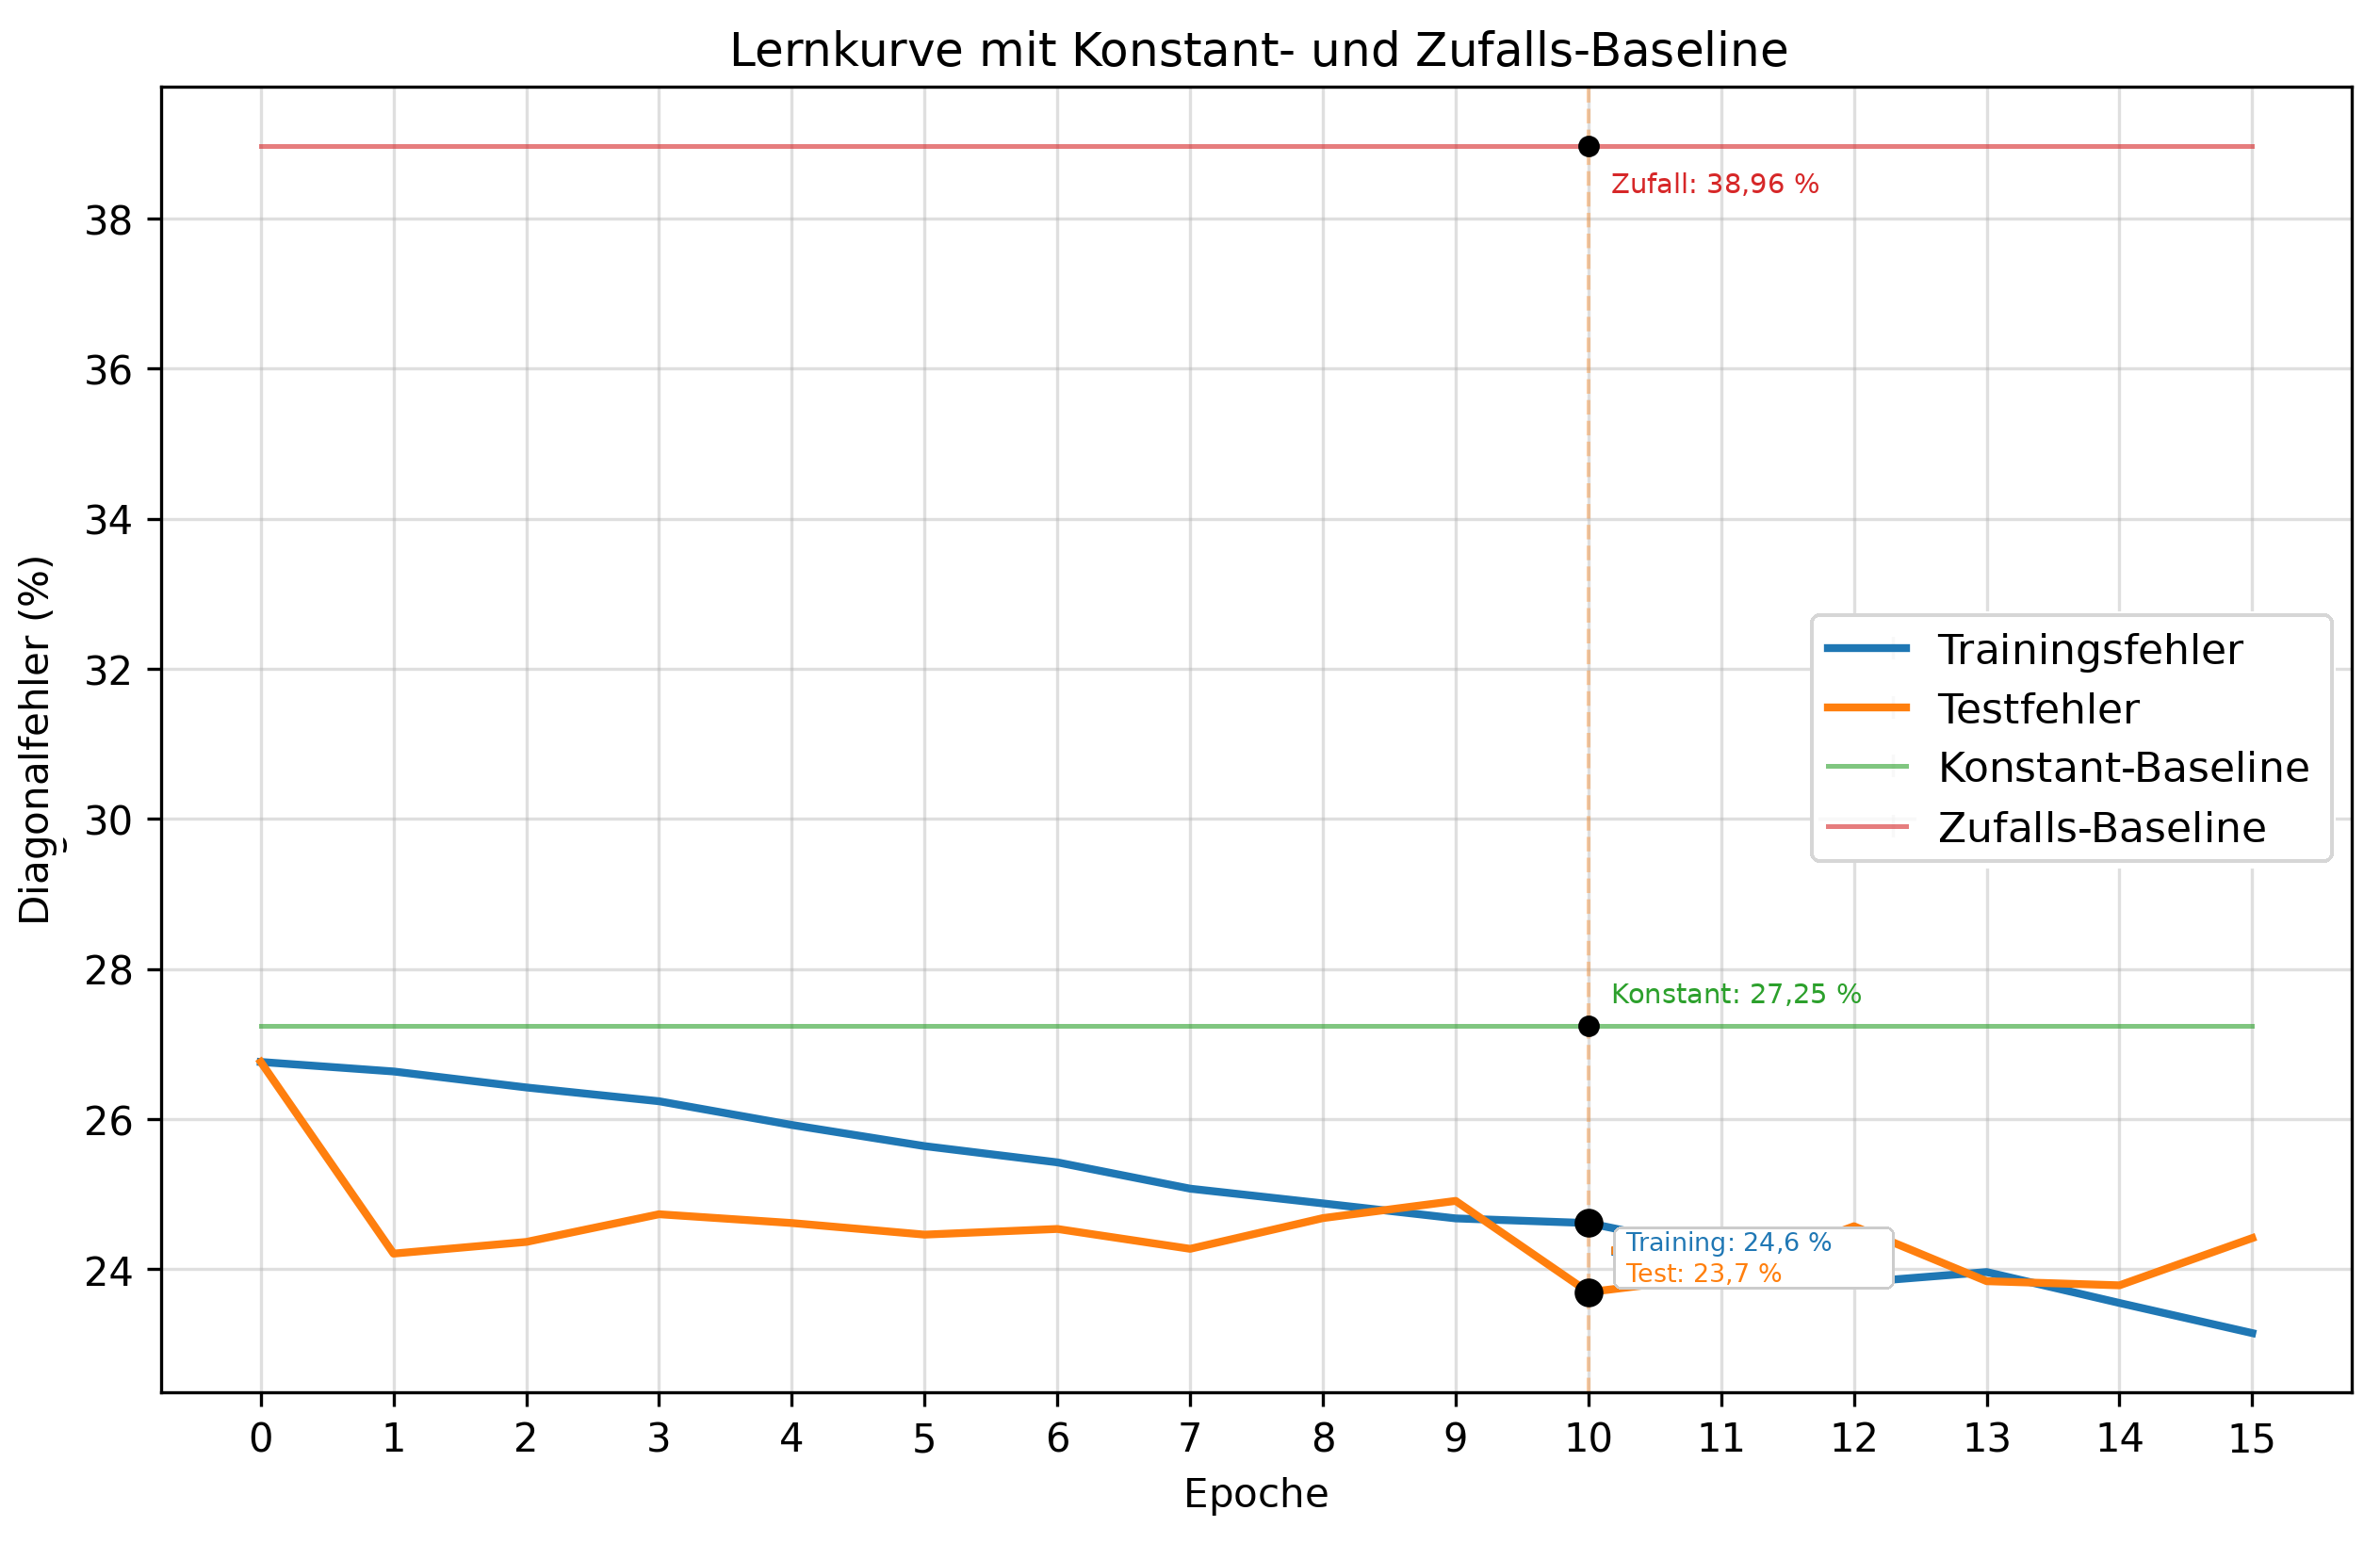
\includegraphics[width=\textwidth]{norm_test_train_const_rand.png}
    \caption[Normierte Ziele]{Normierte Ziele (gleiche Darstellung; gestrichelt:
             Einheitsquadrat). Die hellen Zellen sind Kalibrierpunkte, die auf
             allen Geräten an denselben relativen Stellen gezeigt werden. Unten:
             Lernkurve eines älteren Notebook-Laufs auf \code{norm\_random}
             (\num{1000}/\num{200}, ältere Datenauswahl, siehe
             \cref{sec:data}). Epoch~0 ist das untrainierte Modell. Die
             waagerechten Linien sind fest eingetragene Baselines des
             \emph{gesamten} Datensatzes (27,25\,\% und 38,96\,\%), nicht die
             Baselines der Testdaten dieses Laufs (Konstant-Baseline dort:
             26,76\,\%, siehe Text). Die Werte sind nicht direkt mit den
             Tabellen vergleichbar.}
    \label{fig:normalized_targets}
  \end{subfigure}
  \caption{Rohe und normierte Blickziele im Vergleich.}
  \label{fig:normalization}
\end{figure}

\paragraph{Warum beginnt die Kurve bei der Konstant-Baseline und nicht bei der Zufalls-Baseline?}
In \cref{fig:normalized_targets} beginnen die Kurven in Epoch~0, also
\emph{vor} dem ersten Trainingsschritt, bei \SI{26,77}{\percent}. Man könnte
erwarten, dass ein untrainiertes Modell so schlecht ist wie zufälliges Raten
(etwa \SI{40}{\percent}). Das stimmt aber nicht.

Die Zufalls-Baseline rät für jedes Bild einen \emph{anderen} zufälligen Punkt
auf dem Bildschirm. Ein untrainiertes Netz macht das nicht. Seine Gewichte sind
kleine Zufallszahlen. Die letzte lineare Schicht gibt daher für jedes Bild
Werte nahe $0$ aus, und die Sigmoid macht daraus $\sigma(0)=0,5$. Das
untrainierte Modell sagt also für alle Bilder fast \emph{denselben} Punkt
vorher: die Bildschirmmitte $(0{,}5;\,0{,}5)$. Genau das macht die
Konstant-Baseline. Richtig ist daher:
\begin{itemize}[nosep]
  \item Epoch~0 $\approx$ Konstant-Baseline \emph{derselben} Testdaten
        (\enquote{immer in die Mitte schauen});
  \item erst wenn das Training die Kurve \emph{unter} diesen Wert bringt, hat
        das Modell etwas aus den Bildern gelernt;
  \item die Zufalls-Baseline ist eine obere Grenze für \enquote{reines Raten};
        ein Modell sollte nie darüber liegen.
\end{itemize}
Die Messwerte bestätigen das: Auf den 200 Testbildern dieses Laufs liegt die
Konstant-Baseline bei \SI{26,76}{\percent} (Mittelwert der Trainingsziele) bzw.\
\SI{26,71}{\percent} (Bildschirmmitte). Das entspricht dem Startwert von
\SI{26,77}{\percent}. Wichtig ist, die Baseline auf \emph{denselben} Daten wie
die Kurve zu berechnen. Eine Baseline auf dem gesamten Datensatz
(\SI{27,25}{\percent}) liegt etwas höher, und die Kurve scheint dann
\enquote{unter der Baseline} zu beginnen -- so wie bei der waagerechten Linie
in \cref{fig:normalized_targets}. Der Code berechnet die Baselines
deshalb jetzt auf derselben Teilmenge (\code{metrics.subset\_baselines}).

% ------------------------------------------------------------------------------
\subsection{Baselines}
\label{sec:baselines}

Ich verwende zwei einfache Vergleichsschätzer. Die \emph{Konstant-Baseline}
sagt für jedes Testbild den Mittelwert der Trainingsziele vorher. Die
\emph{Zufalls-Baseline} zieht Vorhersagen gleichverteilt aus $[0,1]^2$. Ein
Modell ist nur dann nützlich, wenn es deutlich besser ist als die
Konstant-Baseline.

\begin{table}[htbp]
  \centering
  \caption[Baseline-Fehler $\Ediag$ in \si{\percent}]{Baseline-Fehler $\Ediag$ in \si{\percent}. Oben: gesamter
           Datensatz (\code{exp.py}, Bootstrap mit 30 Stichproben zu je
           2000 Bildern, Mittelwert und \SI{98}{\percent}-CI). Unten: dieselben
           zufälligen Trainings-/Testteilmengen (Seed 0) wie beim
           Modelltraining (kein CI, eine feste Teilmenge).}
  \label{tab:baselines}
  \small
  \begin{tabular}{lcc}
    \toprule
    Daten & Konstant-Baseline & Zufalls-Baseline \\
    \midrule
    Gesamter Datensatz (\num{347085} Bilder) & 27,28 \,[27,15; 27,40] & 39,82 \,[39,60; 40,04] \\
    \midrule
    \code{norm\_subject}, \num{1000}/\num{200}   & 28,46 & 40,36 \\
    \code{norm\_subject}, \num{10000}/\num{2000} & 27,62 & 39,96 \\
    \code{norm\_random}, \num{1000}/\num{200}    & 27,66 & 39,83 \\
    \bottomrule
  \end{tabular}
\end{table}

Der untere Teil von \cref{tab:baselines} ist die richtige Referenz für alle
Modellergebnisse in \cref{sec:training}, weil er auf denselben Daten berechnet
wurde.

% ==============================================================================
\section{Trainingseinstellungen}
\label{sec:training}
% ==============================================================================

Alle Ergebnisse dieses Abschnitts stammen aus einem Lauf
(\code{exp\_results\_all.json}; \code{exp.py}, korrigierte Metrik, zufällige
Teilmengen mit Seed 0, Early Stopping auf der Validierung, fünf
Wiederholungen pro Einstellung). Die Konstant-Baseline der
Standardeinstellung auf denselben Daten liegt bei \SI{28,46}{\percent}.

% ------------------------------------------------------------------------------
\subsection{Batch Size}
\label{sec:batch}

\begin{table}[htbp]
  \centering
  \caption[Batch Size]{Batch Size. Mittlerer Testfehler über fünf Läufe mit
           \SI{98}{\percent}-CI und mittlere Dauer eines ganzen
           Trainingslaufs (Head auf gespeicherten Features, siehe
           \cref{sec:protocol}).}
  \label{tab:batch_size}
  \small
  \begin{tabular}{ccccc}
    \toprule
    Batch Size & Mittl.\ Testfehler (\%) & \SI{98}{\percent}-CI (\%) & $p$ vs.\ $\dagger$ & Laufzeit (min) \\
    \midrule
    32\sel{}     & 28,39 & [28,21; 28,58] & ---  & 0,019 \\
    64           & 28,35 & [28,29; 28,41] & 0,69 & 0,012 \\
    128          & 28,38 & [28,30; 28,47] & 0,84 & 0,009 \\
    \bottomrule
  \end{tabular}
\end{table}

Die drei Batch Sizes ergeben denselben Testfehler (\cref{tab:batch_size}): Die
Mittelwerte unterscheiden sich um höchstens \num{0,05} Prozentpunkte, die
Confidence Intervals überlappen, und der Rangtest findet keinen Unterschied
($p\ge0,69$). Ein Lauf dauert weniger als eine Sekunde, weil nur der kleine
Head auf gespeicherten Features trainiert wird. Die Zeitunterschiede sind
daher unwichtig.

Ich behalte die Batch Size 32 als Standard. Das Experiment zeigt keinen
Nachteil, und zwei praktische Gründe sprechen für eine kleine Batch Size bei
der Personalisierung: (i) Eine persönliche Sitzung hat nur einige hundert
Trainingsbilder. Mit kleinen Batches gibt es mehr Updates pro Epoch. (ii) Das
Noise kleiner Batches wirkt nach gängiger Meinung leicht regularisierend.
Die Daten dieses Experiments \emph{beweisen} aber keinen Vorteil von 32
gegenüber 64 oder 128.

% ------------------------------------------------------------------------------
\subsection{Learning Rate}
\label{sec:lr}

\begin{table}[htbp]
  \centering
  \caption[Learning Rate]{Learning Rate. Mittlerer Testfehler über fünf Läufe mit
           \SI{98}{\percent}-CI und mittlere Dauer eines ganzen
           Trainingslaufs.}
  \label{tab:learning_rate}
  \small
  \begin{tabular}{ccccc}
    \toprule
    Learning Rate & Mittl.\ Testfehler (\%) & \SI{98}{\percent}-CI (\%) & $p$ vs.\ $\dagger$ & Laufzeit (min) \\
    \midrule
    $10^{-3}$          & 28,43 & [28,33; 28,54] & 0,15  & 0,018 \\
    $10^{-4}$\sel{}    & 28,37 & [28,32; 28,42] & ---   & 0,020 \\
    $10^{-5}$          & 28,33 & [28,28; 28,38] & 0,056 & 0,022 \\
    $10^{-6}$          & 28,37 & [28,21; 28,52] & 0,42  & 0,055 \\
    \bottomrule
  \end{tabular}
\end{table}

\begin{figure}[htbp]
  \centering
  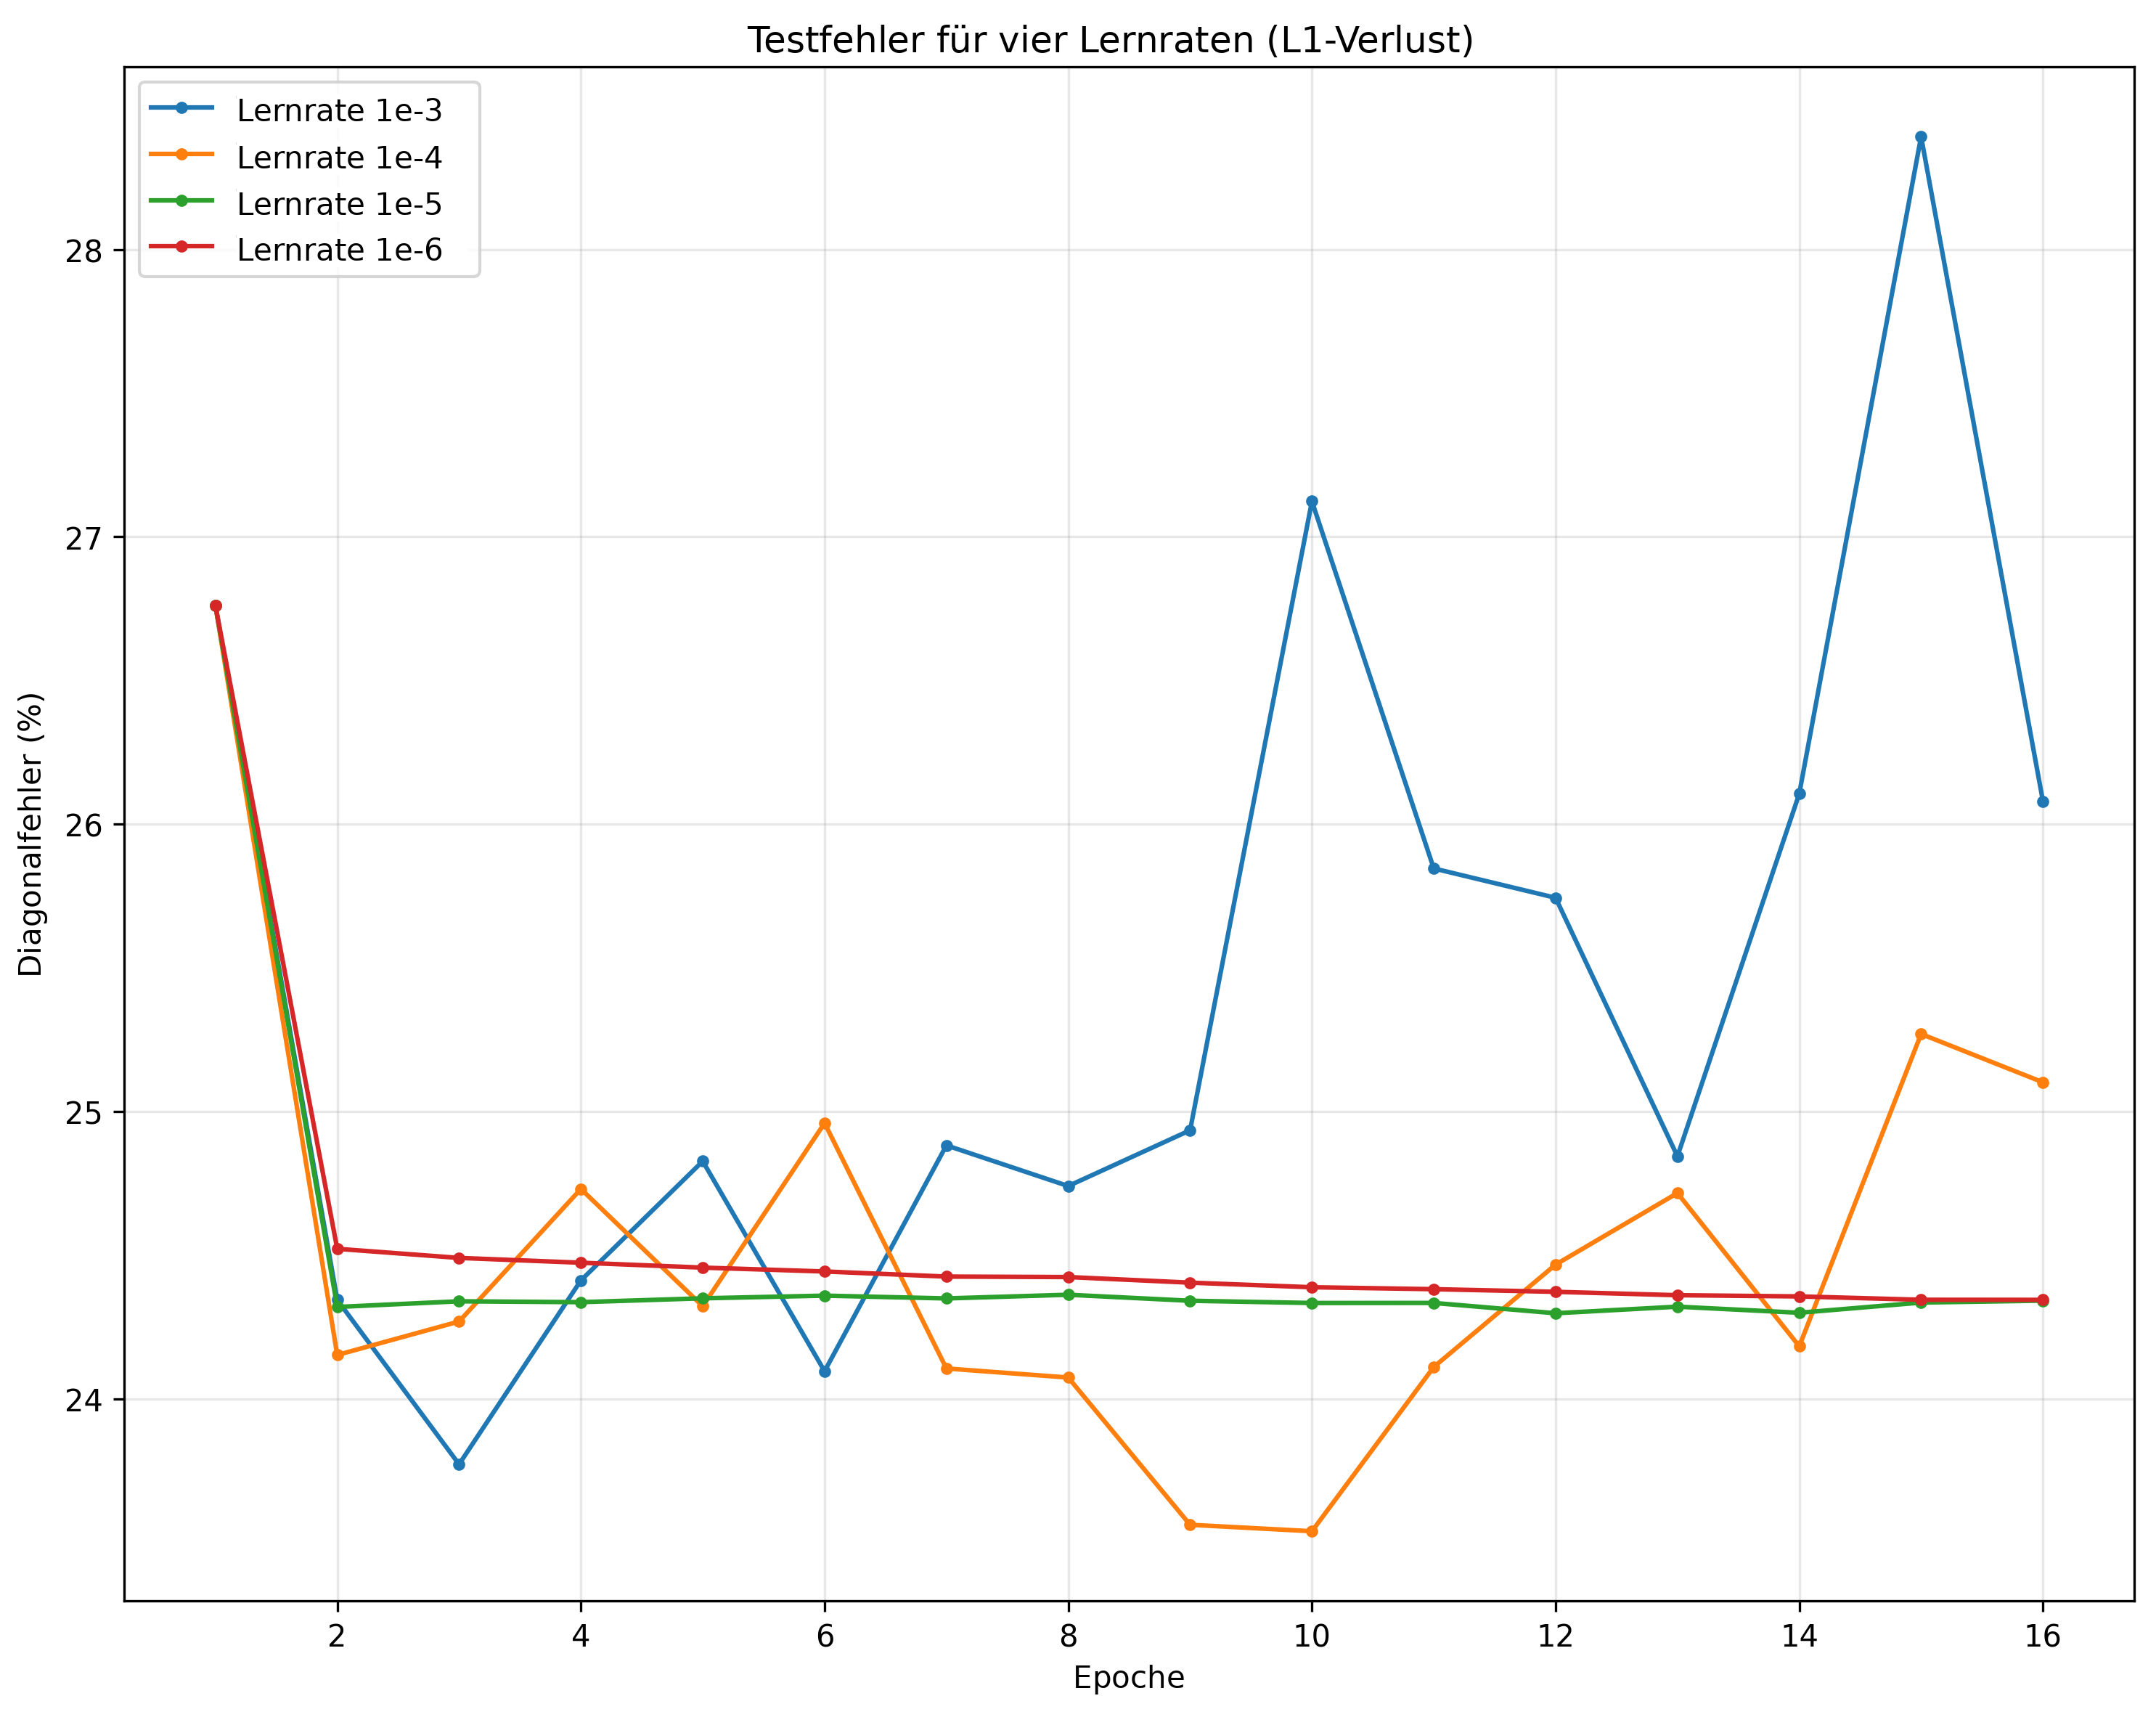
\includegraphics[width=0.78\textwidth]{Test-Error_diff_learning-rate.png}
  \caption[Testfehler einzelner Läufe mit vier Learning Rates]{Testfehler einzelner Trainingsläufe mit vier Learning Rates
           aus einem älteren Notebook-Lauf (\code{norm\_random},
           \num{1000}/\num{200}, ältere Datenauswahl, 15 Epochs ohne Early
           Stopping). Der erste Punkt (Epoch~1 auf der Achse) ist das
           untrainierte Modell. Die Werte sind nicht direkt mit
           \cref{tab:learning_rate} vergleichbar.}
  \label{fig:lr_curves}
\end{figure}

Auch bei der Learning Rate gibt es keinen signifikanten Unterschied
(\cref{tab:learning_rate}): Alle Mittelwerte liegen zwischen
\SI{28,33}{\percent} und \SI{28,43}{\percent}, die Intervalle überlappen, und
kein Rangtest ist signifikant ($p\ge0,056$). Der Endfehler allein kann die
Wahl also nicht begründen. Den Ausschlag gibt der erste Test, also der
\emph{Lernverlauf} in \cref{fig:lr_curves}:
\begin{itemize}[nosep]
  \item $\bm{\eta = 10^{-3}}$: Die Schritte sind zu groß. Nach einem schnellen
        Abfall schwankt der Testfehler stark und steigt wieder (Spitzen bei
        etwa \SI{27,1}{\percent} und \SI{28,4}{\percent}). Der Lauf findet kein
        stabiles Minimum.
  \item $\bm{\eta = 10^{-4}}$: erreicht klar den kleinsten Testfehler aller
        Kurven (etwa \SI{23,6}{\percent} um Epoch~10, also etwa
        0,7~Prozentpunkte unter $10^{-5}$ und $10^{-6}$). Die Kurve schwankt
        noch, aber viel weniger als bei $10^{-3}$. Das Early Stopping kann
        diesen besten Stand behalten.
  \item $\bm{\eta = 10^{-5}}$ \textbf{und} $\bm{10^{-6}}$: Die Kurven sind sehr
        glatt und fallen gleichmäßig, bleiben aber bei etwa
        \SI{24,3}{\percent} stehen. Die Schritte sind zu klein, um in der
        verfügbaren Zeit weiterzukommen. Das Ergebnis ist stabil, aber nicht
        das beste.
\end{itemize}
Auch die Laufzeit spricht für $10^{-4}$ (\cref{tab:learning_rate}): Mit
\SI{0,020}{\min} (etwa \SI{1,2}{\second}) gehört dieser Wert zu den
schnellsten. Nur $10^{-3}$ ist minimal schneller, aber instabil; $10^{-6}$
braucht fast dreimal so lange (\SI{0,055}{\min}), weil das Training mit sehr
kleinen Schritten später abbricht. Ich wähle deshalb $\eta = 10^{-4}$: kleinster
Fehler im ersten Test, ein ruhiger Lernverlauf und eine kurze Laufzeit. Die
Wiederholung mit fünf Läufen zeigt zusätzlich, dass der Head mit gespeicherten
Features robust gegenüber der Learning Rate ist: Keiner der anderen Werte ist
signifikant besser.

% ------------------------------------------------------------------------------
\subsection{Trainierbare Schichten}
\label{sec:layers}

Ich vergleiche drei Tiefen des Fine-Tunings (\cref{tab:params}): nur den
Regression Head (nur FC), den Head plus die letzte Residualstufe
(\code{layer4}) und das ganze Netz.

\begin{table}[htbp]
  \centering
  \caption{Trainierbare Parameter der drei Varianten
           (ResNet-18 mit Regression Head, insgesamt \num{11603650}
           Parameter).}
  \label{tab:params}
  \small
  \begin{tabular}{lrrr}
    \toprule
    & Nur FC & FC + Layer 4 & Volles ResNet \\
    \midrule
    Trainierbare Parameter         & \num{427138} & \num{8820866} & \num{11603650} \\
    Anteil an allen Parametern     & \SI{3,68}{\percent} & \SI{76,02}{\percent} & \SI{100,00}{\percent} \\
    Backbone-Features speicherbar  & ja & nein & nein \\
    \bottomrule
  \end{tabular}
\end{table}

\begin{table}[htbp]
  \centering
  \caption[Trainierbare Schichten]{Trainierbare Schichten. Mittlerer Testfehler über fünf Läufe mit
           \SI{98}{\percent}-CI und mittlere Dauer eines ganzen
           Trainingslaufs. Bei \enquote{nur FC} läuft kein Bild durch den
           Backbone (gespeicherte Features).}
  \label{tab:layers}
  \small
  \begin{tabular}{lcccc}
    \toprule
    Trainierbare Schichten & Mittl.\ Testfehler (\%) & \SI{98}{\percent}-CI (\%) & $p$ vs.\ $\dagger$ & Laufzeit (min) \\
    \midrule
    Nur FC\sel{}           & 28,36 & [28,23; 28,49] & ---  & 0,015 \\
    FC + Layer 4           & 29,07 & [26,58; 31,55] & 0,22 & 9,160 \\
    Volles ResNet          & 29,39 & [26,99; 31,78] & 0,31 & 15,366 \\
    \bottomrule
  \end{tabular}
\end{table}

\enquote{Nur FC} hat den kleinsten mittleren Fehler und mit Abstand das
schmalste Intervall (\cref{tab:layers}). Mehr trainierbare Schichten helfen
nicht. Sie machen das Ergebnis sogar \emph{unsicherer}: Ein Lauf mit FC +
Layer~4 (\SI{31,72}{\percent}) und zwei Läufe mit dem vollen ResNet
(\SI{30,70}{\percent} und \SI{31,18}{\percent}) enden deutlich über der
Konstant-Baseline (\SI{28,46}{\percent}). Alle Läufe mit \enquote{nur FC}
bleiben zwischen \SI{28,28}{\percent} und \SI{28,47}{\percent}. Mit nur fünf
Läufen sind die Unterschiede nicht signifikant ($p=0,22$ und $0,31$); der Wert
für \enquote{nur FC} ist daher nicht fett. Die Trainingszeit wächst stark mit
der Zahl der Parameter: \SI{9,2}{\minute} pro Lauf für FC + Layer~4 und
\SI{15,4}{\minute} für das ganze Netz.

Ich wähle \enquote{nur FC} aus drei Gründen:
\begin{enumerate}[nosep]
  \item \textbf{Nicht schlechter, aber stabiler:} Mehr Schichten senken den
        Fehler hier nicht, sie erhöhen nur die Streuung zwischen den Läufen.
  \item \textbf{Robust bei wenigen Daten:} Eine persönliche Sitzung hat nur
        einige hundert Bilder. Wenn man Millionen von Backbone-Parametern mit
        so wenigen Beispielen trainiert, droht Overfitting, und die
        vortrainierten Features werden verzerrt. \citet{kumar2022finetuning}
        zeigen, dass vollständiges Fine-Tuning vortrainierte Features
        beschädigen und schlechter generalisieren kann als reines
        Head-Training.
  \item \textbf{Aufwand:} Nur \SI{3,68}{\percent} der Parameter werden
        trainiert, und die Backbone-Features werden nur einmal berechnet. Die
        Personalisierung ist dadurch schnell und braucht wenig Speicher.
\end{enumerate}

% ------------------------------------------------------------------------------
\subsection{Activation am Ausgang}
\label{sec:activation}

Die Activation am Ausgang kommt nach der letzten linearen Schicht, die
$(x,y)$ ausgibt. Sigmoid bildet auf $(0,1)$ ab, also genau auf den Bereich der
normierten Koordinaten. Die Gauß-Aktivierung $g(z)=\exp(-z^2/2\sigma^2)$ mit
$\sigma=1$ bildet auf $(0,1]$ ab, ist aber nicht monoton. ReLU entfernt nur
negative Werte, und \enquote{Keine} lässt die Ausgabe unverändert.

\begin{table}[htbp]
  \centering
  \caption[Activation am Ausgang]{Activation am Ausgang. Mittlerer Testfehler über fünf Läufe mit
           \SI{98}{\percent}-CI und mittlere Dauer eines ganzen
           Trainingslaufs.}
  \label{tab:activation}
  \small
  \begin{tabular}{lcccc}
    \toprule
    Activation & Mittl.\ Testfehler (\%) & \SI{98}{\percent}-CI (\%) & $p$ vs.\ $\dagger$ & Laufzeit (min) \\
    \midrule
    Sigmoid\sel{}    & \textbf{28,36} & [28,29; 28,43] & ---   & 0,022 \\
    Gauß             & 31,29 & [28,44; 34,14] & 0,008 & 0,019 \\
    ReLU             & 32,90 & [19,69; 46,10] & 0,008 & 0,028 \\
    Keine            & 29,39 & [28,42; 30,36] & 0,008 & 0,032 \\
    \bottomrule
  \end{tabular}
\end{table}

Sigmoid ist der einzige klare Gewinner der Hyperparameterstudie
(\cref{tab:activation}): kleinster Fehler, schmalstes Intervall, und
\emph{jeder} Sigmoid-Lauf ist besser als \emph{jeder} Lauf der drei anderen
Activations ($p=0,008$ in allen drei Vergleichen). Der Wert ist daher fett.
Die anderen Activations sind auch weniger stabil: Ein ReLU-Lauf endet bei
\SI{46,98}{\percent}, also schlechter als zufälliges Raten. Ein möglicher
Grund: ReLU kann für alle Eingaben null ausgeben (\enquote{tote} Ausgabe), und
der Gradient erholt sich davon nicht mehr. Ohne begrenzende Activation (Keine,
ReLU) kann das Netz außerdem Punkte außerhalb des Bildschirms vorhersagen. Ich
wähle Sigmoid, weil sie die Ausgabe auf den Bildschirm begrenzt und den
kleinsten und stabilsten Fehler ergibt.

% ------------------------------------------------------------------------------
\subsection{Datenmenge}
\label{sec:size}

\begin{table}[htbp]
  \centering
  \caption[Datenmenge (Training/Test)]{Datenmenge (Training/Test). Mittlerer Testfehler über fünf
           Läufe mit \SI{98}{\percent}-CI, mittlere Dauer eines ganzen
           Trainingslaufs und Konstant-Baseline der jeweiligen Testdaten.}
  \label{tab:dataset_size}
  \small
  \setlength{\tabcolsep}{3.5pt}
  \begin{tabular}{lccccc}
    \toprule
    Training / Test & Mittl.\ Testfehler (\%) & \SI{98}{\percent}-CI (\%) & $p$ vs.\ $\dagger$ & Laufzeit (min) & Konst.-Baseline (\%) \\
    \midrule
    \num{10000} / \num{2000}      & 27,64 & [27,55; 27,73] & 0,008 & 0,167 & 27,62 \\
    \num{1000} / \num{200}\sel{}  & 28,39 & [28,33; 28,44] & ---   & 0,018 & 28,46 \\
    \bottomrule
  \end{tabular}
\end{table}

Die größere Datenmenge hat einen kleineren mittleren Fehler
(\cref{tab:dataset_size}). Die beiden Varianten werden aber auf
\emph{verschiedenen} Testdaten ausgewertet, und jeder Mittelwert ist praktisch
gleich der Konstant-Baseline seiner eigenen Testdaten (\SI{27,64}{\percent}
vs.\ \SI{27,62}{\percent} und \SI{28,39}{\percent} vs.\ \SI{28,46}{\percent}).
Der Unterschied von \num{0,75} Prozentpunkten kommt also von den
unterschiedlichen Testdaten und nicht von mehr Trainingsdaten -- auch wenn der
Rangtest signifikant ist ($p=0,008$). Ich behalte die kleine Variante
(\num{1000}/\num{200}), weil sie etwa zehnmal schneller ist und etwa so viele
Daten hat wie eine Personalisierungssitzung.

% ------------------------------------------------------------------------------
\subsection{Art des Splits}
\label{sec:split}

\begin{table}[htbp]
  \centering
  \caption[Art des Splits]{Art des Splits. Mittlerer Testfehler über fünf Läufe mit
           \SI{98}{\percent}-CI und Konstant-Baseline der jeweiligen
           Testdaten.}
  \label{tab:split}
  \small
  \begin{tabular}{lcccc}
    \toprule
    Split & Mittl.\ Testfehler (\%) & \SI{98}{\percent}-CI (\%) & $p$ vs.\ $\dagger$ & Konstant-Baseline (\%) \\
    \midrule
    \code{norm\_random}           & 27,72 & [27,64; 27,80] & 0,008 & 27,66 \\
    \code{norm\_subject}\sel{}    & 28,39 & [28,26; 28,53] & ---   & 28,46 \\
    \bottomrule
  \end{tabular}
\end{table}

Der zufällige Split ergibt den kleineren Fehler (\cref{tab:split}). Auch hier
kommt der größte Teil des Unterschieds von den Testdaten: Die
Konstant-Baseline ist auf \code{norm\_random} schon um \num{0,80}
Prozentpunkte niedriger, und beide Modelle liegen höchstens \num{0,07}
Prozentpunkte neben ihrer Baseline. Außerdem können beim zufälligen Split
dieselben Personen in Training und Test vorkommen. Das macht die Aufgabe
leichter und das Ergebnis zu optimistisch. Ich verwende daher
\code{norm\_subject} als Standard. Nur dieser Split misst die Leistung auf
unbekannten Personen, also die Situation vor der Personalisierung.

% ==============================================================================
\section{Räumliche Fehleranalyse und Loss Functions}
\label{sec:spatial}
% ==============================================================================

Der mittlere Fehler aus \cref{sec:training} zeigt nicht, \emph{wo} auf dem
Bildschirm die Fehler entstehen. Dieser Abschnitt untersucht zuerst die
räumliche Verteilung des Fehlers (\cref{sec:partition,sec:heatmaps}). Das
Ergebnis führte zur Idee, den Loss nach der Position zu gewichten
(\cref{sec:losses}). \Cref{sec:loss_results} wertet diese Idee aus.

\subsection{Einteilung des Bildschirms}
\label{sec:partition}

Ich beschreibe den normierten Bildschirm $[0,1]^2$ mit einem
$3\times3$-Raster aus drei Regionen:
\begin{align*}
  \text{Mitte:}  &\quad (0,50;\,0,50),\\
  \text{Ränder:} &\quad (0,10;\,0,50),\ (0,50;\,0,10),\ (0,90;\,0,50),\ (0,50;\,0,90),\\
  \text{Ecken:}  &\quad (0,10;\,0,10),\ (0,10;\,0,90),\ (0,90;\,0,10),\ (0,90;\,0,90).
\end{align*}
Ein Testbeispiel mit Ziel $\bm p$ gehört zum Rasterpunkt $\bm g$, wenn
$\lVert\bm p-\bm g\rVert_2 \le r$ mit $r = 0,15$ gilt. Der Fehler eines
Rasterpunkts ist der mittlere euklidische Fehler
$\lVert\hat{\bm p}-\bm p\rVert_2$ seiner Beispiele (in normierten Einheiten,
also als Anteil der Bildschirmseite; die Diagonale ist $\sqrt2 \approx 1,41$).
Der Fehler einer Region ist der Mittelwert über alle Beispiele ihrer
Rasterpunkte. Diese Definitionen gelten für alle Abbildungen und Tabellen in
diesem Abschnitt.

\subsection{Fehler-Heatmaps}
\label{sec:heatmaps}

\Cref{fig:heatmaps} nutzt die 200 Testvorhersagen des Standardmodells
(\code{norm\_subject}, L1-Loss; Datei
\code{results/heatmap/base\_loss1.csv}). Für eine Position $\bm c$ (Mitte, Rand
oder Ecke) berechne ich den mittleren Fehler $\bar e(\bm c)$ aller Beispiele im
Radius $r$ und zeichne ihn als Gaußfleck:
\begin{equation}
  H(x,y) = \bar e(\bm c)\,
  \exp\!\left(-\frac{\lVert (x,y)-\bm c\rVert_2^2}{2\sigma^2}\right),
  \qquad \sigma = 0,20 .
\end{equation}
Die Farbe zeigt also die \emph{Größe} des lokalen Fehlers, und die Lage des
hellen Flecks zeigt, \emph{wo} er gemessen wurde. Alle drei Teilbilder nutzen
dieselbe Farbskala (von 0 bis zum größten Wert), damit man die Farben direkt
vergleichen kann.

\begin{figure}[htbp]
  \centering
  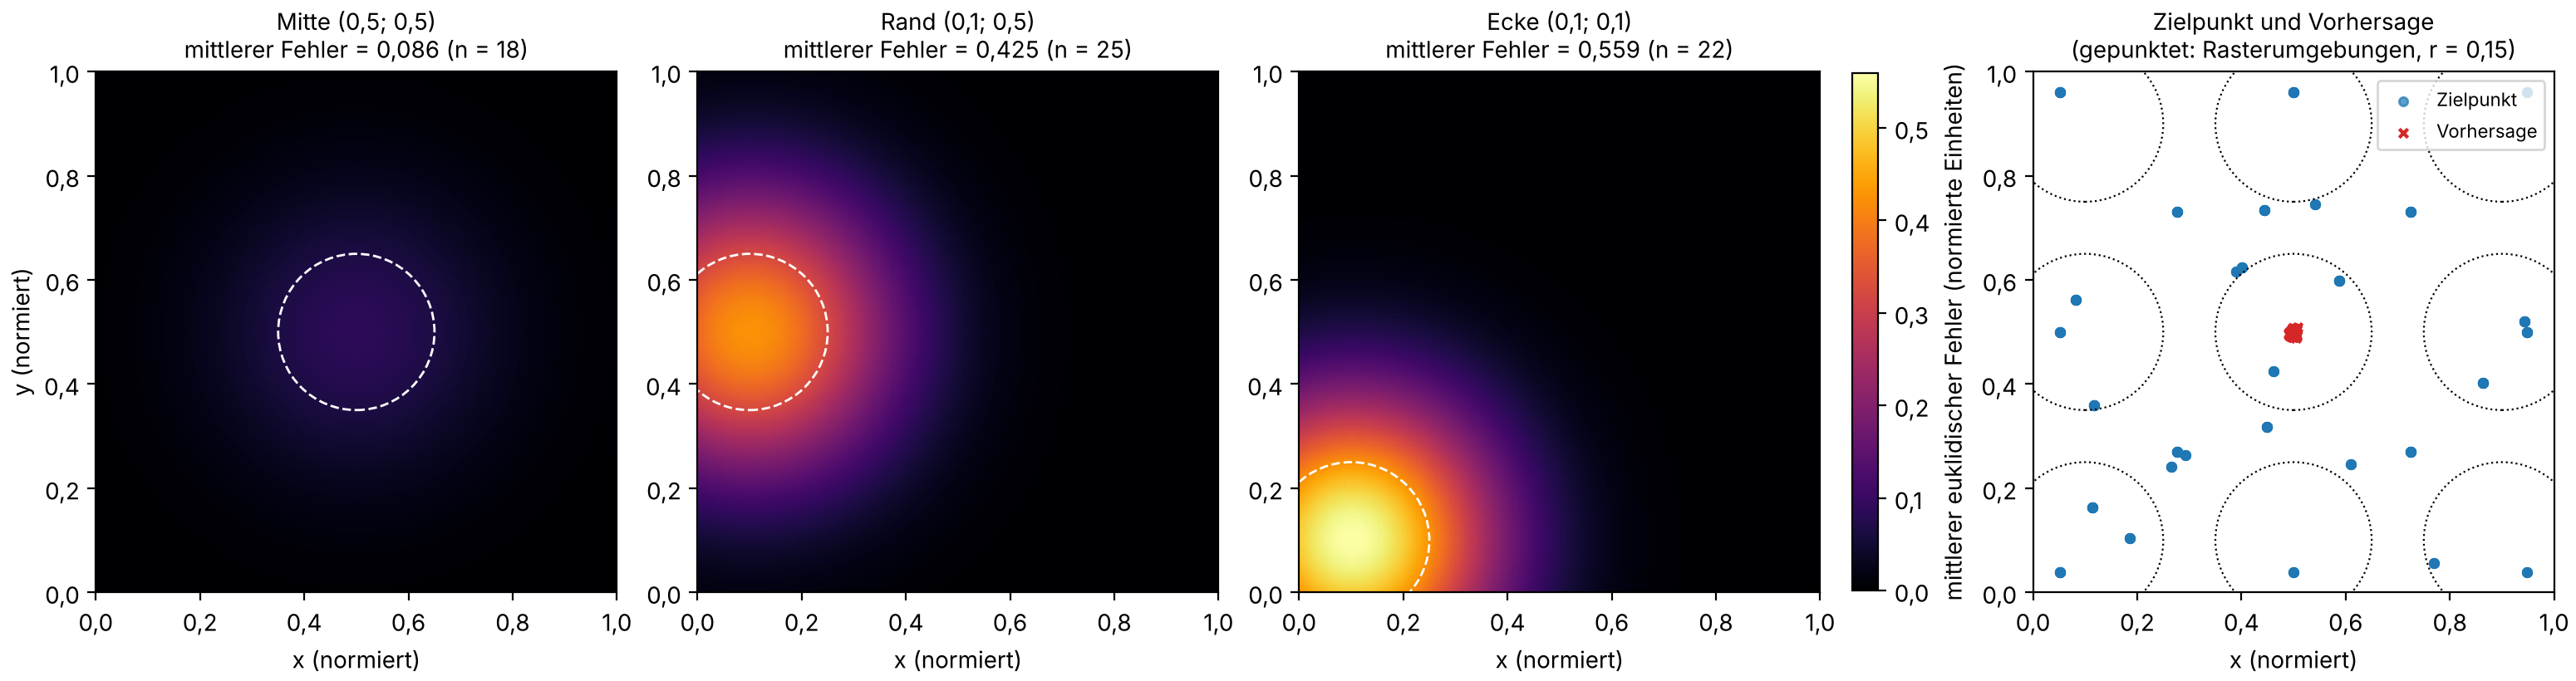
\includegraphics[width=\textwidth]{fig4_spatial_heatmaps.png}
  \caption[Räumlicher Fehler des Standardmodells]{Räumlicher Fehler des Standardmodells (L1-Loss,
           \code{norm\_subject}, 200 Testbeispiele). Teilbilder 1--3:
           Fehler-Heatmaps ($r=0,15$, $\sigma=0,20$, gemeinsame Farbskala) in
           der Mitte $(0,5;\,0,5)$, am linken Rand $(0,1;\,0,5)$ und in der
           unteren linken Ecke $(0,1;\,0,1)$. Der Fehler wächst von der Mitte
           (0,086) über den Rand (0,425) zur Ecke (0,559). Teilbild 4: Ziele
           (blau) und Vorhersagen (rot); alle Vorhersagen liegen nahe der
           Bildschirmmitte.}
  \label{fig:heatmaps}
\end{figure}

Der Fehler wächst von innen nach außen: Er beträgt $0,086$ in der Mitte
($n=18$), $0,432$ an den Rändern ($n=62$) und $0,586$ in den Ecken ($n=42$).
Die Randfehler sind etwa fünfmal und die Eckfehler etwa siebenmal so groß wie
in der Mitte.

Das vierte Teilbild erklärt den Grund. Alle Vorhersagen liegen in einem sehr
kleinen Bereich um $(0,5;\,0,5)$. Ihre Standardabweichung beträgt in beiden
Koordinaten nur etwa $0,004$, die der Ziele dagegen etwa $0,28$. Das Modell
sagt also für jedes Bild fast denselben Punkt vorher. Sein Fehler ist einfach
der Abstand des Ziels von der Bildschirmmitte. Ein Schätzer, der immer die
Mitte ausgibt, liefert praktisch dieselben Werte (Mitte $0,085$, Ränder
$0,432$, Ecken $0,587$; insgesamt $\Ediag=\SI{28,45}{\percent}$ gegenüber
\SI{28,47}{\percent} für das Modell).

\subsection{Loss Functions}
\label{sec:losses}

Wegen der großen Fehler an Rändern und Ecken entstand die Idee, diese Bereiche
im Loss stärker zu gewichten. Sei $\hat{\bm p}_i=(\hat x_i,\hat y_i)$ die
Vorhersage und $\bm p_i=(x_i,y_i)$ das Ziel von Beispiel $i$ in einem Batch der
Größe $N$.

\paragraph{L1-Loss (\code{nn.L1Loss}, \enquote{standard}).}
\begin{equation}
  \mathcal{L}_{1} = \frac{1}{2N}\sum_{i=1}^{N}\bigl(|\hat x_i-x_i| + |\hat y_i-y_i|\bigr).
\end{equation}
Der Gradient hat immer denselben Betrag, egal wie groß der Fehler ist. Der
Loss ist daher robust gegen Ausreißer (zum Beispiel falsche Labels beim
Zielwechsel), behandelt aber alle Bildschirmpositionen gleich.

\paragraph{Smooth-L1-Loss (\code{nn.SmoothL1Loss}, $\beta=1$).}
Für ein Residuum $u$ gilt:
\begin{equation}
  \ell_\beta(u) =
  \begin{cases}
    \dfrac{u^2}{2\beta}, & |u| < \beta,\\[1.2ex]
    |u| - \dfrac{\beta}{2}, & \text{sonst.}
  \end{cases}
\end{equation}
Er ist quadratisch für kleine und linear für große Residuen. Da hier alle
Residuen kleiner als $\beta=1$ sind, verhält er sich wie ein skalierter
quadratischer Fehler: Bei kleinen Fehlern wird der Gradient klein.

\paragraph{Sensitiver L1-Loss (nach Position gewichtet, \code{sensitive}).}
Jedes Beispiel wird mit seinem $L_1$-Abstand zur Bildschirmmitte gewichtet:
\begin{equation}
  d_i = |x_i-0,5| + |y_i-0,5| \in [0,1],\qquad
  w_i = 1 + d_i \in [1,2],
\end{equation}
\begin{equation}
  \mathcal{L}_{\mathrm{sens}} = \frac{1}{N}\sum_{i=1}^{N}
  w_i\cdot\frac{|\hat x_i-x_i| + |\hat y_i-y_i|}{2}.
\end{equation}
Ein Beispiel in der Ecke zählt doppelt so viel wie eines in der Mitte, ein
Beispiel am Rand etwa $1,4$-mal so viel. Der Gradient für äußere Ziele wird
größer, und die Vorhersagen sollen dadurch von der Mitte weggezogen werden.
(Diese Formel entspricht der Implementierung in \code{model.py}.)

Der \enquote{verbesserte sensitive Loss} in \cref{tab:loss_aux} war eine
weitere Variante aus einem Notebook zum Ausprobieren. Seine genaue Formel ist
im aktuellen Code nicht mehr enthalten. Ich nenne ihn nur der Vollständigkeit
halber.

\subsection{Ergebnisse: Vergleich der Loss Functions}
\label{sec:loss_results}

\Cref{tab:loss} zeigt den globalen Vergleich mit fünf Läufen und dazu die
Fehler in den Bildschirmregionen aus \cref{sec:partition}.

\begin{table}[htbp]
  \centering
  \caption[Vergleich von L1- und sensitivem L1-Loss]{Vergleich von L1- und sensitivem L1-Loss. Links: mittlerer
           Testfehler $\Ediag$ über fünf Läufe (\code{exp.py},
           \SI{98}{\percent}-CI) und mittlere Laufzeit. Rechts: mittlerer
           euklidischer Fehler pro Bildschirmregion (normierte Einheiten; je
           ein Lauf, 200 Testbeispiele, $r=0,15$; $n$ = Anzahl der
           Beispiele). Letzte Zeile: Schätzer, der immer die Mitte ausgibt,
           auf denselben 200 Testbeispielen.}
  \label{tab:loss}
  \small
  \setlength{\tabcolsep}{4.5pt}
  \begin{tabular}{lccc@{\hspace{1.2em}}ccc}
    \toprule
    & \multicolumn{3}{c}{Global (5 Läufe)} & \multicolumn{3}{c}{Räumlicher Fehler (1 Lauf)} \\
    \cmidrule(lr){2-4}\cmidrule(lr){5-7}
    Loss & $\Ediag$ (\%) & \SI{98}{\percent}-CI (\%) & Laufzeit (min)
            & Mitte & Ränder & Ecken \\
            &               &                           &
            & ($n=18$) & ($n=62$) & ($n=42$) \\
    \midrule
    L1 (standard)\sel{}    & \textbf{28,32} & [28,23; 28,42] & 0,011 & 0,086 & 0,432 & 0,586 \\
    Sensitiver L1          & 28,48 & [28,19; 28,78] & 0,021 & 0,090 & 0,431 & 0,585 \\
    \midrule
    Konstante Mitte        & 28,45\textsuperscript{a} & --- & --- & 0,085 & 0,432 & 0,587 \\
    \bottomrule
  \end{tabular}\\[1mm]
  \parbox{0.95\linewidth}{\footnotesize \textsuperscript{a}\,Auf denselben 200
  Testbeispielen wie die räumliche Analyse.}
\end{table}

\begin{table}[htbp]
  \centering
  \caption[Zusatzexperiment: räumlicher Fehler von vier Loss Functions]{Zusatzexperiment: räumlicher Fehler von vier Loss Functions nach
           15 Epochs auf Trainingsdaten mit 52 Eckbeispielen (zwei Läufe, A
           und B, Werte wie protokolliert). Die Zahlen stammen aus einem
           Notebook zum Ausprobieren. Die Berechnung der Regionswerte ist im
           aktuellen Code nicht enthalten; sie sind daher nicht direkt mit
           \cref{tab:loss} vergleichbar.}
  \label{tab:loss_aux}
  \small
  \setlength{\tabcolsep}{5pt}
  \begin{tabular}{l cc cc cc cc}
    \toprule
    & \multicolumn{2}{c}{Gesamt (\%)} & \multicolumn{2}{c}{Mitte (\%)}
    & \multicolumn{2}{c}{Ränder (\%)} & \multicolumn{2}{c}{Ecken (\%)} \\
    \cmidrule(lr){2-3}\cmidrule(lr){4-5}\cmidrule(lr){6-7}\cmidrule(lr){8-9}
    Loss & A & B & A & B & A & B & A & B \\
    \midrule
    L1 (\code{nn.L1Loss})             & 24,54 & 24,63 & 17,01 & 16,74 & 28,28 & 28,98 & 34,93 & 35,07 \\
    Smooth L1 (\code{nn.SmoothL1Loss})& 23,94 & 24,91 & 15,40 & 16,41 & 29,78 & 30,59 & 34,13 & 35,17 \\
    Sensitiver L1                     & 25,57 & 25,55 & 19,11 & 18,61 & 29,87 & 29,93 & 33,41 & 34,20 \\
    Verbesserter sensitiver L1        & 25,53 & 27,75 & 19,20 & 21,86 & 29,17 & 35,03 & 33,77 & 31,58 \\
    \bottomrule
  \end{tabular}
\end{table}

\paragraph{Beobachtungen.}
\begin{itemize}[nosep]
  \item Global ist L1 leicht, aber signifikant besser als der sensitive
        Loss: \SI{28,32}{\percent} gegenüber \SI{28,48}{\percent}
        (Mann-Whitney $p=0,032$, \cref{tab:loss}); der L1-Wert ist daher fett.
        Der sensitive Loss streut außerdem stärker zwischen den Läufen.
        Beide Werte liegen nahe an der Konstant-Baseline
        (\SI{28,46}{\percent}).
  \item Räumlich ändert die Gewichtung die Regionsfehler um weniger als
        $0,005$ normierte Einheiten. Rand- und Eckfehler bleiben etwa fünf- bis
        siebenmal so groß wie in der Mitte.
  \item Beide Modelle haben dasselbe räumliche Muster wie ein Schätzer, der
        immer die Mitte ausgibt. Die Gewichtung vergrößert zwar den Gradienten
        für äußere Beispiele, aber das reicht nicht, damit das Modell die Mitte
        verlässt.
  \item Im Zusatzexperiment (\cref{tab:loss_aux}) senken die sensitiven
        Varianten den Eckfehler etwas (sensitiver L1 um
        \num{0,9}--\num{1,5}, die verbesserte Variante um
        \num{1,2}--\num{3,5} Prozentpunkte). Sie erhöhen aber den Fehler in
        der Mitte um \num{1,9}--\num{5,1} Prozentpunkte und den Gesamtfehler in
        allen Läufen. Die beiden Läufe unterscheiden sich stark; diese Tendenzen
        sind daher nicht verlässlich.
\end{itemize}

\paragraph{Fazit.}
Die räumliche Analyse zeigt, \emph{was} das Problem ist: Die Fehler liegen vor
allem an den Rändern und in den Ecken. Der gewichtete Loss sollte diese
Fehler senken. Er hat die Ecken aber nicht verbessert und war global sogar
leicht, aber signifikant schlechter als L1 ($p=0,032$). Im Zusatzexperiment
erhöhte er den Fehler in der Mitte. Ich behalte daher den normalen
L1-Loss: Er hat den kleineren Fehler, ist einfacher, hat keinen
zusätzlichen Parameter, und sein konstanter Gradient macht ihn robust gegen
falsche Labels in den eigenen Aufnahmen. Die Analyse zeigt auch, \emph{warum}
die Gewichtung nicht helfen konnte: Die großen Fehler außen entstehen nicht
durch eine falsche Gewichtung, sondern weil das Modell die Bildschirmmitte
kaum verlässt (\cref{sec:discussion}).

% ==============================================================================
\section{Personalisierungssitzungen}
\label{sec:sessions}
% ==============================================================================

\subsection{Aufbau}
\label{sec:sessions_setup}

In jeder persönlichen Sitzung wird der Head eines GazeCapture-Basismodells
mit den Bildern einer eigenen Aufnahme neu trainiert (nur FC, Sigmoid, L1,
$\eta=10^{-4}$, Weight Decay $10^{-5}$, Batch Size 32, AdamW). Wenn nichts
anderes steht, wird jede Sitzung zufällig in \SI{70}{\percent} Training,
\SI{15}{\percent} Validierung und \SI{15}{\percent} Test geteilt (Seed 42).
Das Early Stopping (Patience 3) nutzt den Validierungsfehler. Ich gebe den
Testfehler in der Epoch mit dem kleinsten Validierungsfehler an. Ist die beste
Epoch~0, hat die Personalisierung die Validierung nicht verbessert. Der
angegebene Testfehler ist dann der des unveränderten Basismodells.

Alle Ergebnisse ab hier stammen aus dem Skript \code{personal\_exp.py}
(Notebook \code{notebooks/Masterarbeit.ipynb}) und verwenden die korrigierte Metrik
(\cref{eq:ediag}). Alle Zufalls-Seeds sind fest. Der Backbone ist einschließlich
seiner BatchNorm-Statistiken vollständig eingefroren.

\paragraph{Feature-Cache.} Weil der Backbone eingefroren ist, liefert er für
ein Bild in jeder Epoch dieselben 512 Features. Ich berechne diese Features
deshalb nur einmal pro Sitzung und Basismodell (ohne Augmentierung) und
speichere sie. Danach wird nur noch der Head trainiert. Das Ergebnis ändert
sich dadurch nicht, aber ein Lauf dauert auf einer CPU nur Sekunden. Der
einzige Unterschied zu älteren Notebook-Läufen: Bei der Personalisierung gibt
es keine Bildaugmentierung.

\paragraph{Basismodelle (E0).} Die beiden Basismodelle werden mit der
Einstellung aus \cref{sec:training} (nur FC, Sigmoid, L1, $\eta=10^{-4}$,
Batch Size 32, \num{1000}/\num{200} zufällige Bilder, Seed~0, Early Stopping
auf der Validierung) auf \code{norm\_subject} und \code{norm\_random}
trainiert. Von fünf Seeds behalte ich jeweils den Lauf mit dem kleinsten
\emph{Validierungs}fehler (\code{train\_base.py},
\code{models/base/base\_<split>.pt}; eine JSON-Datei dokumentiert Einstellung
und alle Seeds). Für \code{norm\_subject} ist das Seed~0 (Validierung
\SI{27,37}{\percent}, Test \SI{28,70}{\percent}; Konstant-Baseline derselben
Testdaten \SI{28,46}{\percent}), für \code{norm\_random} Seed~3 (Validierung
\SI{26,74}{\percent}, Test \SI{27,81}{\percent}; Konstant-Baseline
\SI{27,66}{\percent}). Die fünf Seeds unterscheiden sich um weniger als
\num{0,4} Prozentpunkte; die Wahl des Seeds ist also unkritisch. Wie in
\cref{sec:discussion} beschrieben, liegen beide Basismodelle auf dem Niveau der
Konstant-Baseline.

Von 27 aufgenommenen Sitzungen verwende ich 18: Gen~1 (01--04), Gen~2 (05--09)
und Gen~4 (19--27). Gen~3 (10--18) habe ich verworfen, weil das Modell daraus
nichts lernen konnte. \Cref{tab:session_conditions} zeigt die
Aufnahmebedingungen.

\begin{table}[htbp]
  \centering
  \caption[Aufnahmebedingungen der 18 Sitzungen]{Aufnahmebedingungen der 18 Sitzungen. Gen~1: Ziel bewegt sich
           gleichmäßig, ohne Sprünge; Gen~2: Ziel mit zufälligen Sprüngen;
           Gen~4: 5-s-Abschnitte (\SI{0,5}{\second} WAIT an einem neuen
           Startpunkt, \SI{4,5}{\second} MOVE), \SI{90}{\percent} der
           Startpunkte in den Ecken. Die Dauer wurde nur in Gen~4 verändert
           (Gen~1/2: nicht protokolliert). Gerät~A: Sitzungen 01--03 und
           25--27; Gerät~B: 05--09 und 19--24; Sitzung 04: nicht protokolliert.}
  \label{tab:session_conditions}
  \small
  \begin{tabular}{llll}
    \toprule
    Sitzungen & Generation & Brille & Licht / Hintergrund \\
    \midrule
    01, 03, 04 & Gen 1 & mit    & 01, 04: hell; 03: dunkel \\
    02         & Gen 1 & ohne   & hell \\
    05, 07, 08 & Gen 2 & mit    & 05: hell; 07: dunkel; 08: sehr dunkel \\
    06, 09     & Gen 2 & ohne   & 06: hell; 09: sehr dunkel \\
    \midrule
    \multicolumn{4}{l}{Gen 4 \quad (Dauer / Gerät)} \\
    19, 20 & Gen 4 & mit    & ruhig; 120\,s / 90\,s; B \\
    21, 22 & Gen 4 & ohne   & ruhig; 120\,s / 90\,s; B \\
    23 / 24 & Gen 4 & mit / ohne & unruhig; 120\,s; B \\
    25 / 26 & Gen 4 & mit / ohne & unruhig; 120\,s; A \\
    27     & Gen 4 & mit    & unruhig; 90\,s; A \\
    \bottomrule
  \end{tabular}
\end{table}

\subsection{Ergebnisse aller Sitzungen (E1)}
\label{sec:sessions_results}

\Cref{tab:sessions} zeigt jede Sitzung mit beiden Basismodellen.

\begin{table}[htbp]
  \centering
  \caption[Personalisierung der 18 Sitzungen mit zwei Basismodellen]{Personalisierung der 18 Sitzungen mit zwei Basismodellen
           (ursprüngliche Labels, zufälliger 70/15/15-Split, Seed 42). Basis:
           Testfehler des unveränderten Basismodells (Epoch~0); Val.:
           bester Validierungsfehler; Test: Testfehler in der besten
           Validierungsepoche; Ep.: beste Epoch; $t$: Dauer eines Laufs in
           Sekunden (\cref{sec:session_time}); Konst.: Konstant-Baseline
           (Mittelwert der Trainingsziele, auf denselben Testbildern). Fehler
           in \si{\percent} (\cref{eq:ediag}). Gruppenzeilen: Mittelwert und
           \SI{98}{\percent}-CI über die Sitzungen der Gruppe.}
  \label{tab:sessions}
  \footnotesize
  \setlength{\tabcolsep}{2.6pt}
  \resizebox{\textwidth}{!}{%
  \begin{tabular}{cc ccccc ccccc c}
    \toprule
    & & \multicolumn{5}{c}{Basismodell \code{norm\_subject}}
      & \multicolumn{5}{c}{Basismodell \code{norm\_random}} & \\
    \cmidrule(lr){3-7}\cmidrule(lr){8-12}
    Sitzung & Gen. & Basis & Val. & Test & Ep. & $t$ (s) & Basis & Val. & Test & Ep. & $t$ (s) & Konst. \\
    \midrule
    01 & 1 & 29,19 & 14,82 & 15,83 & 22 & 2,3 & 29,49 & 11,70 & 12,97 & 47 & 4,2 & 29,45 \\
    02 & 1 & 28,48 & 10,08 & 10,48 & 30 & 2,2 & 28,42 & 10,04 & 10,43 & 44 & 3,2 & 28,49 \\
    03 & 1 & 29,61 & 15,26 & 17,20 & 33 & 2,5 & 30,13 & 15,41 & 17,35 & 36 & 2,6 & 29,76 \\
    04 & 1 & 29,98 & 16,88 & 17,64 & 17 & 2,1 & 29,38 & 15,23 & 16,16 & 31 & 2,7 & 29,17 \\
    05 & 2 & 32,92 & 25,43 & 17,64 & 26 & 1,1 & 32,49 & 31,93 & 32,77 & 2 & 0,2 & 32,72 \\
    06 & 2 & 29,29 & 11,31 & 16,67 & 54 & 1,8 & 28,89 & 12,09 & 16,55 & 55 & 2,0 & 27,02 \\
    07 & 2 & 32,18 & 24,84 & 30,99 & 16 & 0,7 & 32,43 & 25,02 & 31,62 & 18 & 0,6 & 32,28 \\
    08 & 2 & 25,82 & 23,65 & 23,30 & 24 & 0,8 & 26,32 & 23,38 & 22,31 & 23 & 0,6 & 27,00 \\
    09 & 2 & 26,83 & 23,55 & 28,64 & 4 & 0,2 & 26,21 & 15,19 & 16,87 & 47 & 1,9 & 28,17 \\
    19 & 4 & 30,42 & 13,38 & 17,76 & 33 & 2,8 & 30,04 & 12,13 & 16,85 & 47 & 4,4 & 30,19 \\
    20 & 4 & 33,14 & 16,06 & 14,64 & 23 & 1,9 & 33,01 & 14,58 & 12,93 & 35 & 2,7 & 33,49 \\
    21 & 4 & 30,18 & 15,03 & 12,51 & 39 & 4,6 & 30,46 & 15,80 & 13,20 & 23 & 2,6 & 29,97 \\
    22 & 4 & 31,17 & 13,54 & 13,02 & 22 & 2,2 & 30,87 & 12,53 & 12,32 & 37 & 3,1 & 30,32 \\
    23 & 4 & 33,15 & 23,48 & 23,65 & 10 & 1,4 & 32,59 & 24,02 & 24,05 & 10 & 2,0 & 32,57 \\
    24 & 4 & 33,09 & 28,77 & 26,97 & 7 & 0,9 & 32,84 & 29,53 & 27,42 & 6 & 1,0 & 33,01 \\
    25 & 4 & 32,19 & 26,98 & 24,61 & 19 & 2,4 & 33,00 & 26,74 & 24,13 & 26 & 2,8 & 31,54 \\
    26 & 4 & 30,60 & 21,93 & 18,61 & 20 & 2,3 & 30,39 & 21,40 & 17,97 & 37 & 4,5 & 29,48 \\
    27 & 4 & 31,98 & 26,05 & 26,06 & 19 & 1,5 & 32,29 & 26,27 & 26,68 & 19 & 1,7 & 31,19 \\
    \midrule
    \multicolumn{2}{l}{Gen 1 (4)} & 29,32 & 14,26 & 15,29 & 25,5 & 2,3 & 29,35 & 13,10 & 14,23 & 39,5 & 3,2 & 29,22 \\
      & & [27,86; 30,77] & [7,62; 20,89] & [7,80; 22,77] & & [1,8; 2,7] & [27,75; 30,96] & [7,07; 19,12] & [7,10; 21,35] & & [1,5; 4,8] & [27,99; 30,45] \\
    \multicolumn{2}{l}{Gen 2 (5)} & 29,41 & 21,76 & 23,45 & 24,8 & 0,9 & 29,27 & 21,52 & 24,02 & 29,0 & 1,0 & 29,44 \\
      & & [24,14; 34,68] & [11,88; 31,63] & [12,74; 34,16] & & [0,0; 1,9]\textsuperscript{a} & [24,06; 34,47] & [8,20; 34,85] & [10,93; 37,12] & & [0,0; 2,5]\textsuperscript{a} & [24,68; 34,20] \\
    \multicolumn{2}{l}{Gen 4 (9)} & 31,77 & 20,58 & 19,76 & 21,3 & 2,2 & 31,72 & 20,33 & 19,51 & 26,7 & 2,8 & 31,31 \\
      & & [30,60; 32,94] & [14,66; 26,50] & [14,26; 25,26] & & [1,2; 3,3] & [30,51; 32,93] & [13,88; 26,79] & [13,59; 25,42] & & [1,7; 3,9] & [29,91; 32,70] \\
    \midrule
    \multicolumn{2}{l}{\textbf{Alle (18)}} & \textbf{30,57} & \textbf{19,50} & \textbf{19,79} & \textbf{23,2} & \textbf{1,9} & \textbf{30,51} & \textbf{19,05} & \textbf{19,59} & \textbf{30,2} & \textbf{2,4} & \textbf{30,32} \\
      & & [29,27; 31,87] & [15,87; 23,13] & [16,18; 23,40] & & [1,3; 2,5] & [29,21; 31,82] & [14,86; 23,25] & [15,47; 23,71] & & [1,6; 3,2] & [29,12; 31,53] \\
    \bottomrule
  \end{tabular}}\\[1mm]
  \parbox{0.95\linewidth}{\footnotesize \textsuperscript{a}\,Die untere Grenze
  des $t$-Intervalls liegt unter null (wenige Sitzungen, große Streuung) und
  wurde bei 0 abgeschnitten.}
\end{table}

\begin{figure}[htbp]
  \centering
  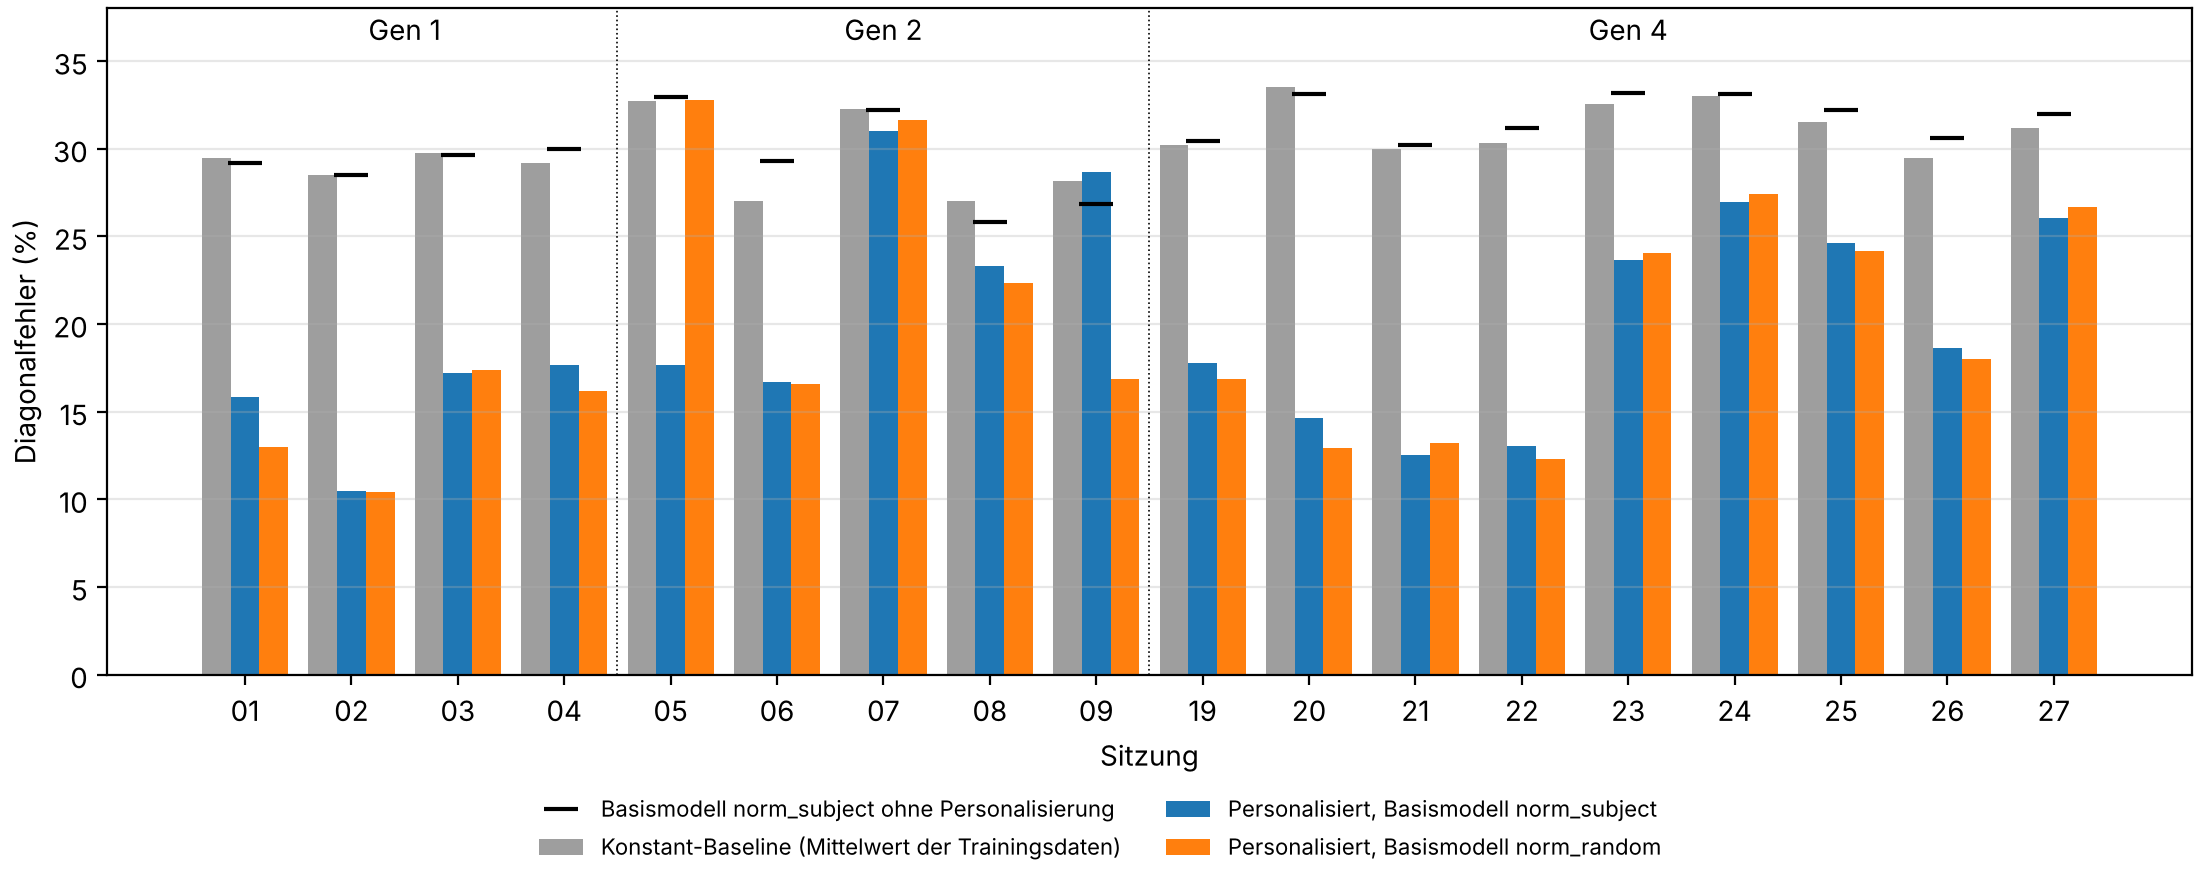
\includegraphics[width=\textwidth]{fig_sessions_baseline.png}
  \caption{Testfehler der 18 Sitzungen nach der Personalisierung mit beiden
           Basismodellen, verglichen mit der Konstant-Baseline und dem
           unveränderten Basismodell (\code{norm\_subject}) auf denselben
           Testbildern (Daten aus \cref{tab:sessions}).}
  \label{fig:sessions}
\end{figure}

\paragraph{Die Personalisierung funktioniert.}
Über alle 18 Sitzungen sinkt der Testfehler von \SI{30,32}{\percent}
(Konstant-Baseline) auf \SI{19,79}{\percent} mit dem Basismodell
\code{norm\_subject} und auf \SI{19,59}{\percent} mit dem Basismodell
\code{norm\_random}. Das ist eine Verringerung um \SI{35}{\percent} bzw.\
\SI{36}{\percent} (Wilcoxon-Vorzeichen-Rang-Test $p=1,5\cdot10^{-5}$ für beide;
gepaarter $t$-Test $p<10^{-6}$). Die unveränderten Basismodelle sind nicht
besser als die Konstant-Baseline (\SI{30,57}{\percent} und
\SI{30,51}{\percent}; Wilcoxon $p=0,25$ und $p=0,35$). Der ganze Gewinn kommt
also aus den wenigen Minuten persönlicher Daten. Die beste Sitzung, S02 (Gen~1,
heller Raum, ohne Brille), erreicht \SI{10,5}{\percent}. Die neuen Läufe
bestätigen die älteren Notebook-Läufe (Mittelwert \SI{19,85}{\percent} über
dieselben Sitzungen mit \code{norm\_subject}).

\paragraph{Gruppen.} Gegenüber der Konstant-Baseline sinkt der Fehler um
\SI{48}{\percent} / \SI{51}{\percent} in Gen~1, um \SI{20}{\percent} /
\SI{18}{\percent} in Gen~2 und um \SI{37}{\percent} / \SI{38}{\percent} in
Gen~4 (\code{norm\_subject} / \code{norm\_random}). In Gen~4 ist die
Verbesserung signifikant (Wilcoxon $p=0,004$). Für Gen~1 ($n=4$) und Gen~2
($n=5$) ist der kleinste mögliche $p$-Wert dieses Tests $0,125$ bzw.\
$0,0625$. Diese Gruppen sind also zu klein für ein signifikantes Ergebnis,
obwohl der Effekt in Gen~1 groß ist. Die Unterschiede zwischen den Generationen
sind nicht signifikant (Kruskal-Wallis $p=0,13$ und $p=0,12$). Man darf sie
nicht allein als Wirkung des Aufnahmeablaufs deuten
(\cref{sec:session_design}).

\paragraph{Wenn die Personalisierung scheitert.}
In zwei Läufen ist das personalisierte Modell nicht besser als die
Konstant-Baseline: S09 mit \code{norm\_subject} (beste Epoch~4,
\SI{28,64}{\percent} gegenüber \SI{28,17}{\percent}) und S05 mit
\code{norm\_random} (beste Epoch~2, \SI{32,77}{\percent} gegenüber
\SI{32,72}{\percent}). In beiden Fällen hat sich der Validierungsfehler sehr
früh nicht mehr verbessert. Mit dem jeweils anderen Basismodell erreichen
dieselben Sitzungen \SI{16,87}{\percent} (S09) und \SI{17,64}{\percent} (S05).
Das Scheitern liegt also nicht an der Sitzung, sondern an einem einzelnen Lauf:
Mit nur 20 bis 30 Validierungsbildern (Gen~2) kann das Early Stopping das
Training schon nach wenigen Epochs beenden. S07 (dunkler Raum) verbessert sich
mit beiden Basismodellen nur wenig (\SI{31,0}{\percent} /
\SI{31,6}{\percent} gegenüber \SI{32,3}{\percent}). Gutes Licht bleibt also eine
Voraussetzung für die Personalisierung mit Webcam.

\paragraph{Basismodell.}
Beide Basismodelle ergeben dasselbe Ergebnis (\SI{19,79}{\percent} gegenüber
\SI{19,59}{\percent}; Wilcoxon $p=0,20$). Das passt zum Hauptergebnis: Das
Basismodell liefert vor allem einen Startpunkt, und die persönlichen Daten
bestimmen das Ergebnis. In den folgenden Experimenten verwende ich das
Basismodell \code{norm\_subject}, weil es ohne Information über die
Testpersonen trainiert wurde.

\paragraph{Validierungs- und Testfehler.} Im Mittel liegt der
Validierungsfehler (\SI{19,50}{\percent}) nahe am Testfehler
(\SI{19,79}{\percent}). Die größten Abweichungen (5 bis 8 Prozentpunkte, S05
bis S07, S09) gibt es bei den kurzen Gen-2-Aufnahmen. Dort haben Validierung
und Test jeweils nur etwa 25 Bilder.

\subsection{Trainingszeit einer Sitzung}
\label{sec:session_time}

Die Zeit $t$ in \cref{tab:sessions} ist die echte Dauer \emph{eines ganzen
Personalisierungslaufs} auf den gespeicherten Features: Auswertung des
unveränderten Modells (Epoch~0), alle Epochs bis zum Early Stopping und nach
jeder Epoch die Auswertung auf Trainings-, Validierungs- und Testdaten. Sie
ist weder eine Zeit pro Epoch noch ein Mittelwert über mehrere Läufe. Sie
enthält nicht die einmalige Berechnung der Backbone-Features der Sitzung. Ein
Lauf dauert auf einer CPU im Mittel \SI{1,9}{\second} (\code{norm\_subject})
bzw.\ \SI{2,4}{\second} (\code{norm\_random}). Die Dauer wächst mit der Zahl
der Bilder und der Epochs (kurze Gen-2-Aufnahmen: \SI{0,9}{\second}). Ältere
Notebook-Läufe, die jedes Bild in jeder Epoch durch den Backbone schickten,
brauchten 1 bis 26 Minuten pro Sitzung. Die \enquote{Laufzeit} in den
Hyperparametertabellen (\cref{sec:protocol}) ist dagegen ein Mittelwert über
fünf Läufe einer GazeCapture-Einstellung.

\subsection{Bereinigung der Labels (Gen 4, E1b)}
\label{sec:cleaning}

In Gen~4 beginnt jeder Abschnitt mit einer WAIT-Phase von \SI{0,5}{\second}.
Das Ziel erscheint an einer neuen Stelle, und der Nutzer muss es erst finden.
Diese Bilder (\SI{10,0}{} bis \SI{10,5}{\percent} der Labels) können ein
falsches Blicklabel haben. Weil sie genau protokolliert sind, kann man
bereinigte Labeldateien ohne WAIT-Bilder schreiben
(\code{session\_design.py --write-clean}).

Ein einfacher Vergleich wäre aber unfair: Das bereinigte Modell wird ohne
WAIT-Bilder getestet, das ursprüngliche Modell dagegen mit allen Bildern,
also auch mit den schwer vorhersagbaren WAIT-Bildern. Deshalb werte ich das
ursprüngliche Modell zusätzlich nur auf den MOVE-Bildern seiner Testdaten aus
(gleiches Modell, WAIT-Bilder aus dem Test entfernt; \cref{tab:cleaning}).

\begin{table}[htbp]
  \centering
  \caption[Bereinigung der Labels in Gen~4]{Bereinigung der Labels in Gen~4 (Basismodell \code{norm\_subject},
           zufälliger Split, Seed 42). Ursprünglich: mit allen Labels
           trainiert; Testfehler auf allen Testbildern, nur auf MOVE und nur
           auf WAIT ($n_W$ = Anzahl der WAIT-Testbilder). Bereinigt: ohne
           WAIT-Bilder trainiert und getestet. $\Delta$ = Bereinigt $-$
           Ursprünglich (MOVE).}
  \label{tab:cleaning}
  \footnotesize
  \setlength{\tabcolsep}{4pt}
  \begin{tabular}{c cccc cc c}
    \toprule
    & \multicolumn{4}{c}{Ursprüngliche Labels} & \multicolumn{2}{c}{Bereinigte Labels} & \\
    \cmidrule(lr){2-5}\cmidrule(lr){6-7}
    Sitzung & Alle & MOVE & WAIT & $n_W$ & Test & Konst. & $\Delta$ \\
    \midrule
    19 & 17,76 & 13,28 & 41,12 & 8  & 13,06 & 29,07 & $-0,22$ \\
    20 & 14,64 & 12,24 & 28,38 & 8  & 12,77 & 30,71 & $+0,53$ \\
    21 & 12,51 &  9,77 & 27,59 & 10 &  9,79 & 29,23 & $+0,01$ \\
    22 & 13,02 & 10,21 & 27,64 & 8  &  9,96 & 31,71 & $-0,25$ \\
    23 & 23,65 & 20,95 & 41,84 & 10 & 17,18 & 30,92 & $-3,77$ \\
    24 & 26,97 & 24,96 & 41,93 & 10 & 23,99 & 31,64 & $-0,97$ \\
    25 & 24,61 & 21,63 & 44,36 & 10 & 17,94 & 30,49 & $-3,70$ \\
    26 & 18,61 & 14,34 & 41,72 & 10 & 14,58 & 30,20 & $+0,24$ \\
    27 & 26,06 & 23,10 & 44,80 & 8  & 23,69 & 30,59 & $+0,60$ \\
    \midrule
    Mittel & 19,76 & 16,72 & 37,71 & 9,1 & 15,88 & 30,51 & $-0,84$ \\
    \bottomrule
  \end{tabular}
\end{table}

\paragraph{Ergebnis.} Die WAIT-Bilder werden sehr schlecht vorhergesagt
(\SI{37,7}{\percent}, schlechter als die Konstant-Baseline). Der Blick ist noch
nicht auf dem Ziel, ihre Labels sind also falsch. Entfernt man sie nur aus den
\emph{Test}daten, sinkt der Fehler von \SI{19,76}{\percent} auf
\SI{16,72}{\percent}. Entfernt man sie auch aus den \emph{Trainings}daten,
sinkt er weiter auf \SI{15,88}{\percent}. Dieser Gewinn von \num{0,84}
Prozentpunkten ist nicht signifikant (Wilcoxon $p=0,43$). Er kommt von zwei
Sitzungen mit unruhigem Hintergrund (S23, S25, je etwa $-3,7$ Punkte). In den
ruhigen Sitzungen ist der Unterschied kleiner als \num{0,6} Punkte. Fazit: Die
WAIT-Bilder sollte man mindestens aus der Auswertung entfernen, weil sie den
Fehler der Labels messen und nicht den Fehler des Modells. Sie auch aus dem
Training zu entfernen, kostet nichts und hilft in schwierigen Sitzungen; der
Effekt ist aber klein.

\paragraph{Schwankung zwischen Läufen.} Zwei ältere Notebook-Läufe mit
gleicher Einstellung auf denselben Daten (Gen~4, Seeds nicht fest)
unterschieden sich im Mittel um \num{1,9} und höchstens um \num{5,5}
Prozentpunkte. Die neuen Läufe mit drei festen Seeds (\cref{tab:loading})
zeigen eine Standardabweichung von bis zu \num{3,1} Prozentpunkten zwischen den
Seeds. Unterschiede zwischen \emph{einzelnen} Läufen in dieser Größe kann man
also nicht deuten. Das erklärt auch die Fälle S05 und S09 oben.

\subsection{Aufnahmebedingungen (Gen 4)}
\label{sec:conditions}

In Gen~4 kann man Sitzungen vergleichen, die sich nur in einem Faktor
unterscheiden. Jeder Wert ist die Differenz zweier einzelner Sitzungen
(Testfehler aus \cref{tab:sessions}, \code{norm\_subject} /
\code{norm\_random}, in Prozentpunkten; positiv bedeutet: die erste Bedingung
ist schlechter):
\begin{itemize}[nosep]
  \item \textbf{Brille} (mit $-$ ohne): $+5,2/+3,6$ (S19--S21),
        $+1,6/+0,6$ (S20--S22), $-3,3/-3,4$ (S23--S24), $+6,0/+6,2$ (S25--S26);
  \item \textbf{Dauer} (\SI{90}{\second} $-$ \SI{120}{\second}):
        $-3,1/-3,9$ (S20--S19), $+0,5/-0,9$ (S22--S21);
  \item \textbf{Hintergrund} (unruhig $-$ ruhig): $+5,9/+7,2$ (S23--S19),
        $+14,5/+14,2$ (S24--S21);
  \item \textbf{Gerät} (A $-$ B, verschiedene Webcams): $+1,0/+0,1$
        (S25--S23), $-8,4/-9,4$ (S26--S24).
\end{itemize}
Der einzige einheitliche und große Effekt ist der \textbf{Hintergrund}: Ein
unruhiger Hintergrund erhöht den Fehler mit beiden Basismodellen um 6 bis 15
Prozentpunkte. Eine Brille erhöht den Fehler meistens (drei von vier Paaren).
Die Dauer (90 vs.\ 120\,s) zeigt keinen klaren Effekt, und der Vergleich der
beiden Geräte ist widersprüchlich. Jede Bedingung kommt nur in einzelnen
Sitzungen vor. Diese Werte beschreiben also nur, sie sind nicht statistisch
getestet.

% ==============================================================================
\section{Strategien zum Aufteilen der Daten (E2)}
\label{sec:loading}
% ==============================================================================

Der zufällige Split aus \cref{sec:sessions} hat eine Schwäche: Benachbarte
Bilder eines Videos sind fast gleich (6 Labels pro Sekunde). Die Testdaten
enthalten also fast exakte Kopien von Trainingsbildern. Das ist ein Datenleck
(Data Leakage), und es macht den zufälligen Split zu optimistisch. Der
folgende Vergleich misst, wie groß dieser Effekt ist.

\paragraph{Sitzungen.} Ich verwende die Sitzungen 21 und 22. Ich wähle sie
nach einer festen Regel: Sie sind die einzigen zwei Sitzungen, die sich nur in
einem Faktor unterscheiden (Dauer \SI{120}{\second} vs.\ \SI{90}{\second}).
Sonst wurden sie unter den besten Bedingungen aufgenommen (Gen~4, ohne Brille,
ruhiger Hintergrund, gleiches Gerät, gleicher Tag). Sie eignen sich daher für den
Transfer zwischen zwei Videos, und beide haben genug Bilder (720 und 540) für
zeitliche Blöcke.

\paragraph{Strategien.}
\begin{description}[nosep]
  \item[Zufällig] (\code{--split random}): \SI{70}{\percent} /
        \SI{15}{\percent} / \SI{15}{\percent} der Bilder werden zufällig
        gezogen (Referenz; enthält fast gleiche Bilder in Training und Test).
  \item[Sequenziell] (\code{--split sequential}): Die Bilder bleiben in der
        Reihenfolge der Aufnahme. Die ersten \SI{70}{\percent} sind Training,
        die nächsten \SI{15}{\percent} Validierung und die letzten
        \SI{15}{\percent} Test. Am Anfang des Validierungs- und des Testblocks
        wird jeweils eine Sekunde (6 Labels) weggelassen, damit keine
        Nachbarbilder auf beiden Seiten einer Grenze liegen. Das entspricht der
        echten Nutzung: Der Nutzer kalibriert zuerst und benutzt den Tracker
        danach.
  \item[Zwei Videos] (\code{--split two\_videos}): \SI{80}{\percent} der
        Bilder der ersten Sitzung sind Training, die übrigen \SI{20}{\percent}
        (zufällig) Validierung. Die zweite Sitzung dient \emph{nur} als Test
        (alle Bilder). Ich teste beide Richtungen (21$\to$22 und 22$\to$21).
        So sieht man, ob eine Kalibrierung auch für eine neue Aufnahme
        derselben Person gilt.
\end{description}

\paragraph{Fairer Vergleich.} Alle Strategien verwenden dasselbe Basismodell
(\code{norm\_subject}), dieselben Trainingseinstellungen, Early Stopping auf
ihren eigenen Validierungsdaten und dieselben drei Seeds (42, 43, 44). Für
jeden Lauf gebe ich die Konstant-Baseline (Mittelwert der
\emph{Trainings}ziele, ausgewertet auf den Testbildern dieses Laufs) und den
Fehler des unveränderten Basismodells auf denselben Testbildern an. So kann man
die verschiedenen Testdaten vergleichen. Kein Testbild wird für Training oder
Modellauswahl verwendet.

\begin{table}[htbp]
  \centering
  \caption[Strategien zum Aufteilen der Daten]{Strategien zum Aufteilen der Daten (Sitzungen 21 und 22,
           Basismodell \code{norm\_subject}, ursprüngliche Labels). Mittelwert
           über drei Seeds; SD: Standardabweichung des Testfehlers über die
           Seeds; Basis: unverändertes Basismodell; Red.: Verringerung des
           Testfehlers gegenüber der Konstant-Baseline; $n$: Trainings- /
           Validierungs- / Testbilder; $t$: Dauer eines Laufs (s).}
  \label{tab:loading}
  \footnotesize
  \setlength{\tabcolsep}{3.5pt}
  \resizebox{\textwidth}{!}{%
  \begin{tabular}{l c cc c cc c c c}
    \toprule
    Strategie & Training $\to$ Test & Test (\%) & SD & Val.\ (\%) & Basis (\%) & Konst.\ (\%) & Red.\ (\%) & $n$ & $t$ (s) \\
    \midrule
    Zufällig    & 21 $\to$ 21 & 14,40 & 3,13 & 14,15 & 31,52 & 31,25 & 53,9 & 503 / 108 / 109 & 3,9 \\
                & 22 $\to$ 22 & 13,30 & 0,38 & 15,98 & 30,97 & 30,68 & 56,7 & 378 / 81 / 81   & 3,1 \\
    Sequenziell & 21 $\to$ 21 & 14,47 & 1,22 & 19,09 & 27,62 & 27,43 & 47,2 & 503 / 102 / 103 & 2,0 \\
                & 22 $\to$ 22 & 16,63 & 0,14 & 14,41 & 28,83 & 29,91 & 44,4 & 378 / 75 / 75   & 2,4 \\
    Zwei Videos & 21 $\to$ 22 & 16,79 & 0,13 & 15,67 & 31,05 & 32,17 & 47,8 & 576 / 144 / 540 & 5,0 \\
                & 22 $\to$ 21 & 17,70 & 0,42 & 14,33 & 32,03 & 33,13 & 46,6 & 432 / 108 / 720 & 3,2 \\
    \midrule
    \multicolumn{2}{l}{Zufällig (Mittel)}    & 13,85 & & & 31,25 & 30,97 & 55,3 & & \\
    \multicolumn{2}{l}{Sequenziell (Mittel)} & 15,55 & & & 28,22 & 28,67 & 45,8 & & \\
    \multicolumn{2}{l}{Zwei Videos (Mittel)} & 17,24 & & & 31,54 & 32,65 & 47,2 & & \\
    \bottomrule
  \end{tabular}}
\end{table}

\paragraph{Ergebnis.} Die erwartete Reihenfolge stimmt: zufällig
(\SI{13,85}{\percent}) $<$ sequenziell (\SI{15,55}{\percent}) $<$ zwei Videos
(\SI{17,24}{\percent}). Mit 6 Läufen pro Strategie (zwei Sitzungen $\times$
drei Seeds) ist nur der Unterschied zwischen sequenziell und zwei Videos
signifikant (Mann-Whitney U, $p=0,009$). Zufällig vs.\ sequenziell ($p=0,09$)
und zufällig vs.\ zwei Videos ($p=0,06$) sind es nicht. Weil die
Konstant-Baselines der Testdaten verschieden sind, ist die relative
Verringerung das fairere Maß: \SI{55}{\percent} beim zufälligen Split, aber nur
\SI{46}{\percent} bis \SI{47}{\percent} bei den realistischen Strategien. Der
zufällige Split überschätzt den Nutzen der Personalisierung also um etwa 8 bis
9 Prozentpunkte der Verringerung.

\paragraph{Deutung.}
\begin{itemize}[nosep]
  \item Der zufällige Split ist zu optimistisch, bei diesen beiden guten
        Sitzungen aber nur mäßig (1,7 Prozentpunkte). Bei schwierigen
        Sitzungen ist der Effekt viel größer (\cref{sec:design_performance}).
  \item Eine Kalibrierung funktioniert auch für eine zweite Aufnahme derselben
        Person unter denselben Bedingungen: Auf einem nie gesehenen Video
        erreicht das Modell \SI{17}{\percent} bis \SI{18}{\percent} bei
        \SI{47}{\percent} Verringerung. Der Transfer kostet gegenüber dem
        zufälligen Split etwa 3 Prozentpunkte.
  \item Die Ergebnisse mit zwei Videos schwanken am wenigsten zwischen den
        Seeds (SD unter 0,5), weil die Testdaten groß sind (540 bis 720
        Bilder). Der zufällige Split schwankt am meisten (SD 3,1 bei S21), weil
        seine 81 bis 109 Testbilder vom Seed abhängen.
  \item Beim sequenziellen Split sagt der Validierungsfehler den Testfehler
        schlecht voraus (S21: \SI{19,1}{\percent} Validierung vs.\
        \SI{14,5}{\percent} Test). Validierungs- und Testblock zeigen
        verschiedene Bereiche des Bildschirms.
\end{itemize}
Für einen Eye-Tracker, der einmal kalibriert und danach benutzt wird, sind die
Werte des sequenziellen Splits und der zwei Videos die realistische Schätzung.

% ==============================================================================
\section{Gestaltung der Kalibriersitzung}
\label{sec:session_design}
% ==============================================================================

Die Gestaltung der Sitzung bestimmt, welche Bildschirmbereiche die
Kalibrierdaten abdecken. Weil die Fehler an Rändern und Ecken am größten sind
(\cref{sec:spatial}), soll die Gestaltung diese Bereiche gut abdecken. Ich
habe drei Varianten aufgenommen:
\begin{itemize}[nosep]
  \item \textbf{Standardvideo} (Gen~1, \code{base\_Code.py}): Das Ziel bewegt
        sich gleichmäßig und ohne Sprünge über den Bildschirm;
  \item \textbf{Zufällige Sprünge} (Gen~2): Das Ziel springt alle
        \SI{1,4}{} bis \SI{2,7}{\second} an einen zufälligen neuen
        Startpunkt;
  \item \textbf{Ecken-gewichtete Sprünge} (Gen~4, \code{base\_Code\_rand.py}):
        5-s-Abschnitte mit \SI{0,5}{\second} WAIT an einem neuen Startpunkt und
        \SI{4,5}{\second} MOVE; \SI{90}{\percent} der Startpunkte liegen in den
        vier Eckbereichen (je \SI{10}{\percent}\,$\times$\,\SI{10}{\percent}
        des Bildschirms).
\end{itemize}

\subsection{Abdeckung des Bildschirms und Transition Frames}

\Cref{tab:design} wird direkt aus den Label- und Positionsdateien der 18
Sitzungen berechnet (\code{session\_design.py}); dafür ist kein Training nötig.
Die Anteile der Regionen nutzen die Einteilung aus \cref{sec:partition}
($r=0,15$). Transition Frames sind Labels, die aufgenommen wurden, während der
Blick noch zum neuen Ziel wandert: in Gen~4 die protokollierte WAIT-Phase, in
Gen~2 die Labels bis \SI{0,5}{\second} nach einem Sprung (geschätzt, ohne
Phasenprotokoll), in Gen~1 keine.

\begin{table}[htbp]
  \centering
  \caption[Abdeckung und Transition Frames pro Gestaltung]{Abdeckung des Bildschirms und Transition Frames pro Gestaltung
           (Mittelwert über die Sitzungen jeder Generation). Zellen: Anteil
           der 100 Zellen eines $10\times10$-Rasters mit mindestens einem
           Label; Abst.: mittlerer Abstand der Ziele von der Bildschirmmitte
           (normierte Einheiten).}
  \label{tab:design}
  \small
  \setlength{\tabcolsep}{4pt}
  \resizebox{\textwidth}{!}{%
  \begin{tabular}{l c c c c ccc c c}
    \toprule
    Gestaltung & Labels & Länge & Sprünge & Übergang & \multicolumn{3}{c}{Anteil der Labels (\%)} & Zellen & Abst. \\
    \cmidrule(lr){6-8}
               &        & (s)   &         & (\%)     & Mitte & Ränder & Ecken & (\%) & \\
    \midrule
    Standard (Gen 1, 4 Sitz.)          & 493 & 82  & 0  & 0           & 7,1 & 25,0 & 23,0 & 97 & 0,383 \\
    Zufällige Sprünge (Gen 2, 5 Sitz.) & 179 & 30  & 16 & 28,5\textsuperscript{a} & 6,3 & 23,0 & 26,3 & 57 & 0,384 \\
    Ecken-gewichtet (Gen 4, 9 Sitz.)   & 644 & 107 & 20 & 10,1        & 6,1 & 19,5 & 36,1 & 91 & 0,420 \\
    \bottomrule
  \end{tabular}}\\[1mm]
  \parbox{0.95\linewidth}{\footnotesize \textsuperscript{a}\,Geschätzt:
  Labels bis \SI{0,5}{\second} nach einem Sprung.}
\end{table}

\paragraph{Beobachtungen.}
\begin{itemize}[nosep]
  \item \textbf{Die Gewichtung der Ecken wirkt wie geplant:} Gen~4 hat
        \SI{36}{\percent} seiner Labels in der Nähe der Ecken, Gen~1 nur
        \SI{23}{\percent} und Gen~2 \SI{26}{\percent}. Gen~4 hat auch den
        größten mittleren Abstand von der Mitte.
  \item \textbf{Eine gleichmäßige Bewegung deckt den Bildschirm am besten
        ab:} Gen~1 erreicht \SI{97}{\percent} der Rasterzellen. Die kurzen
        Gen-2-Aufnahmen (\SI{30}{\second}) decken nur \SI{57}{\percent} ab.
  \item \textbf{Transition Frames:} Mit Sprüngen alle 1,4 bis 2,7 Sekunden und
        ohne Phasenprotokoll fallen im Mittel etwa \SI{28,5}{\percent} der Gen-2-Labels in einen
        Übergang (geschätzt). Gen~4 hat \SI{10}{\percent}; diese sind genau protokolliert
        und können entfernt werden (\cref{sec:cleaning}).
\end{itemize}

\subsection{Ergebnis der Personalisierung (E3)}
\label{sec:design_performance}

Der zufällige Split bevorzugt Gestaltungen mit langsamer, gleichmäßiger
Bewegung, weil fast gleiche Nachbarbilder in Training und Test landen. Deshalb
habe ich alle 18 Sitzungen zusätzlich mit dem sequenziellen Split trainiert
(\cref{sec:loading}; Basismodell \code{norm\_subject}, Seed 42).
\Cref{tab:design_perf} vergleicht beide Splits pro Gestaltung.
\Cref{tab:region_errors} zeigt die Fehler pro Bildschirmregion, berechnet aus
den gespeicherten Testvorhersagen.

\begin{table}[htbp]
  \centering
  \caption[Testfehler pro Gestaltung mit zufälligem und sequenziellem Split]{Testfehler pro Gestaltung mit zufälligem und sequenziellem Split
           (Mittelwert über die Sitzungen; Basismodell \code{norm\_subject}).
           Konst.: Konstant-Baseline der jeweiligen Testbilder; Ep.~0: Anzahl
           der Sitzungen mit bester Epoch~0 (keine Verbesserung gegenüber dem
           Basismodell); $n_{\text{Test}}$: mittlere Anzahl der Testbilder.}
  \label{tab:design_perf}
  \footnotesize
  \setlength{\tabcolsep}{4pt}
  \begin{tabular}{l cc cccc}
    \toprule
    & \multicolumn{2}{c}{Zufälliger Split} & \multicolumn{4}{c}{Sequenzieller Split} \\
    \cmidrule(lr){2-3}\cmidrule(lr){4-7}
    Gestaltung & Test & Konst. & Test & Konst. & Ep.~0 & $n_{\text{Test}}$ \\
    \midrule
    Standard (Gen 1)          & 15,29 & 29,22 & 21,52 & 28,70 & 1 / 4 & 69 \\
    Zufällige Sprünge (Gen 2) & 23,45 & 29,44 & 32,80 & 34,39 & 2 / 5 & 22 \\
    Ecken-gewichtet (Gen 4)   & 19,76 & 31,31 & 28,07 & 31,82 & 5 / 9 & 91 \\
    \midrule
    Alle (18)                 & 19,79 & 30,32 & 27,93 & 31,84\textsuperscript{a} & 8 / 18 & 67 \\
    \bottomrule
  \end{tabular}\\[1mm]
  \parbox{0.9\linewidth}{\footnotesize \textsuperscript{a}\,Mittelwert der
  Sitzungswerte des sequenziellen Splits.}
\end{table}

\begin{table}[htbp]
  \centering
  \caption[Testfehler pro Bildschirmregion]{Testfehler pro Bildschirmregion (\cref{sec:partition}, $r=0,15$),
           Mittelwert über die Sitzungen einer Gestaltung; in Klammern die
           Gesamtzahl der Testbilder in der Region. Basismodell
           \code{norm\_subject}.}
  \label{tab:region_errors}
  \footnotesize
  \setlength{\tabcolsep}{3.5pt}
  \resizebox{\textwidth}{!}{%
  \begin{tabular}{l cccc cccc}
    \toprule
    & \multicolumn{4}{c}{Zufälliger Split} & \multicolumn{4}{c}{Sequenzieller Split} \\
    \cmidrule(lr){2-5}\cmidrule(lr){6-9}
    Gestaltung & Alle & Mitte & Ränder & Ecken & Alle & Mitte & Ränder & Ecken \\
    \midrule
    Standard (Gen 1)          & 15,3 & 17,7 (20) & 13,5 (67) & 16,7 (83)  & 21,5 & 11,9 (25) & 20,9 (64)  & 28,9 (52) \\
    Zufällige Sprünge (Gen 2) & 23,4 & 13,7 (12) & 21,6 (34) & 26,1 (42)  & 32,8 & 6,6 (2)\textsuperscript{a} & 29,8 (15) & 38,6 (45) \\
    Ecken-gewichtet (Gen 4)   & 19,8 & 11,5 (45) & 14,9 (175) & 26,5 (299) & 28,1 & 9,0 (60) & 23,9 (136) & 37,1 (289) \\
    \midrule
    Alle (18)                 & 19,8 & 13,5 (77) & 16,4 (276) & 24,2 (424) & 27,9 & 9,7 (87) & 24,3 (215) & 36,1 (386) \\
    \bottomrule
  \end{tabular}}\\[1mm]
  \parbox{0.95\linewidth}{\footnotesize \textsuperscript{a}\,Nur eine Sitzung
  mit zwei Bildern in der Mitte; nicht aussagekräftig.}
\end{table}

\paragraph{Sequenzieller Split.} Ohne fast gleiche Bilder in Training und
Test steigt der Fehler bei jeder Gestaltung, im Mittel von \SI{19,8}{\percent}
auf \SI{27,9}{\percent} (Wilcoxon $p=4\cdot10^{-5}$). Das personalisierte
Modell ist immer noch besser als die Konstant-Baseline (Wilcoxon $p=0,002$),
aber die Verringerung schrumpft von \SI{35}{\percent} auf etwa
\SI{12}{\percent}. In 8 von 18 Sitzungen (02, 05, 08, 23--27) ist die beste
Epoch~0: Training auf den ersten \SI{70}{\percent} der Aufnahme verbessert den
Fehler auf dem Validierungsblock nicht. Das angegebene Ergebnis ist dann das
unveränderte Basismodell. Das passiert vor allem in Gen~4 mit unruhigem
Hintergrund (23--27) und bei den kurzen Gen-2-Aufnahmen, deren Validierungs-
und Testblöcke nur 17 bis 27 Bilder haben. Der zufällige Split aus
\cref{sec:sessions} überschätzt den Nutzen der Personalisierung bei
schwierigen Sitzungen also stark.

\paragraph{Gestaltungen.} Bei beiden Splits hat das Standardvideo (Gen~1) den
kleinsten und die zufälligen Sprünge (Gen~2) den größten Fehler. Auch mit dem
sequenziellen Split sind die Unterschiede nicht signifikant (Kruskal-Wallis
$p=0,06$). Die Reihenfolge lässt sich durch die Abdeckung erklären
(\cref{tab:design}): Gen~1 deckt in jedem Teil der Aufnahme \SI{97}{\percent}
des Bildschirms ab. Bei den Sprung-Gestaltungen deckt ein zeitlicher Block nur
die Ziele ab, die in dieser Zeit gezeigt wurden. Die kurzen Gen-2-Aufnahmen
leiden am meisten darunter. Die Gestaltungen sind außerdem mit Licht,
Hintergrund und Brille vermischt. Die Reihenfolge ist also eine Tendenz, kein
Beweis.

\paragraph{Regionen.} Die Ecken sind bei jeder Gestaltung und bei beiden
Splits am schwierigsten (\SI{24}{\percent} zufällig, \SI{36}{\percent}
sequenziell), die Mitte am leichtesten (\SI{10}{} bis \SI{14}{\percent}). Die
Ecken-gewichtete Gestaltung senkt den Eckfehler \emph{nicht}: Gen~4 hat
\SI{26,5}{\percent} / \SI{37,1}{\percent} in den Ecken, das Standardvideo
\SI{16,7}{\percent} / \SI{28,9}{\percent}. Mehr Ecklabels allein helfen also
nicht, wenn der Blick in den Ecken schwerer zu schätzen ist (Kopfdrehung, halb
geschlossene Augen, Lage der Kamera) und wenn die Ecklabels unter schlechteren
Bedingungen aufgenommen wurden (Gen-4-Sitzungen 23--27). Außerdem muss die
Sigmoid-Ausgabe in den äußersten Ecken nahe 0 oder 1 liegen.

\paragraph{Folgerung für die Gestaltung.} Mit den vorhandenen Daten liefert
für eine kurze Kalibrierung eine gleichmäßige Zielbewegung über den ganzen
Bildschirm das beste Ergebnis. Sprünge erzeugen Transition Frames (Gen~2: im Mittel etwa
\SI{28,5}{\percent} der Labels). Wenn man Sprünge verwendet, muss man sie
protokollieren, damit man diese Bilder entfernen kann. Die Gewichtung der Ecken
erhöht den Anteil der Ecklabels wie geplant, senkt aber nicht den Eckfehler.

% ==============================================================================
\section{Diskussion der Ergebnisse}
\label{sec:discussion}
% ==============================================================================

\paragraph{Hauptergebnis.}
Auf GazeCapture erreichen alle Einstellungen der Hyperparameterstudie
praktisch nur den Fehler eines konstanten Schätzers auf denselben Testdaten:
Die besten Einstellungen mit \enquote{nur FC} liegen zwischen
\SI{28,32}{\percent} und \SI{28,39}{\percent}, die Konstant-Baseline bei
\SI{28,46}{\percent}. Die räumliche Analyse bestätigt, dass die Vorhersagen
in der Bildschirmmitte liegen. Die Hyperparameterstudie trennt die
Einstellungen daher vor allem nach ihrer \emph{Stabilität}: Optionen, die das
Training unruhiger machen (Gauß, ReLU, keine Activation, mehr trainierbare
Schichten, sensitiver Loss), sind schlechter. Aber keine Option verlässt
deutlich die Mitte. Die Entscheidungen in \cref{sec:training} beruhen daher
auf Stabilität, Lernverlauf, Aufwand und methodischen Gründen, wie in jedem
Unterabschnitt beschrieben. Einzelne Notebook-Läufe auf \code{norm\_random}
(\cref{fig:lr_curves,fig:normalized_targets}) erreichten zwar etwa
\SI{23,6}{\percent} bei einer Konstant-Baseline von \SI{26,8}{\percent} auf
ihren Testdaten. Diese Läufe nutzten aber eine ältere Datenauswahl. Mit dem
aktuellen Protokoll (zufällige Datenauswahl, fünf Läufe) ist ein solcher
Lerneffekt nicht sichtbar. Die älteren Werte sind daher kein Beleg für einen
Lerneffekt. Die Basismodelle bestätigen das: Ihr Fehler auf den persönlichen
Sitzungen (\SI{30,6}{\percent}) entspricht der Konstant-Baseline.

\paragraph{Mögliche Ursachen.} Zwei Erklärungen kann das neue Protokoll
bereits ausschließen: Die Trainingsdaten enthalten jetzt 179 statt fünf
Personen, und die Testdaten werden nicht mehr für die Modellauswahl verwendet.
Trotzdem bleiben die Vorhersagen in der Mitte. Die wahrscheinlichsten Ursachen
sind:
(i) Ich verwende ganze Kamerabilder. Die Augen sind darin nur ein kleiner Teil
des Bildes. Die eingefrorenen ImageNet-Features enthalten daher wenig
Blickinformation.
(ii) \num{1000} Bilder von 179 Personen sind nur etwa sechs Bilder pro Person.
Das ist zu wenig, um eine Abbildung für alle Personen zu lernen. Mehr
trainierbare Schichten mit so wenigen Daten machen das Training nur instabil
(\cref{sec:layers}).
Gesichts- oder Augenausschnitte als Eingabe und mehr Trainingsdaten sind die
nächsten Schritte, die man prüfen sollte.

\paragraph{Personalisierung.}
Mit demselben eingefrorenen Backbone senkt ein Head, der auf einigen hundert
Bildern einer Person trainiert wurde, den Fehler gegenüber der
Konstant-Baseline. Mit einem zeitlichen Split, der der echten Nutzung
entspricht, beträgt die Verringerung im Mittel etwa \SI{12}{\percent}
(\SI{31,8}{\percent} $\rightarrow$ \SI{27,9}{\percent}) und in schwierigen
Sitzungen null. Gute Sitzungen behalten aber den größten Teil des Gewinns, und
eine Kalibrierung funktioniert sogar für eine zweite Aufnahme
(\SI{47}{\percent} Verringerung, \cref{sec:loading}). Der zufällige Split
zeigt eine Verringerung um etwa ein Drittel, ist aber zu optimistisch. Ein Lauf
dauert auf einer CPU etwa zwei Sekunden, und die Wahl des Basismodells spielt
keine Rolle; es liefert vor allem einen Startpunkt. Das unterstützt die zentrale
Idee dieser Arbeit, die dateneffiziente Personalisierung eines vortrainierten
Modells. Wichtig ist außerdem: Die Aufnahmebedingungen (Hintergrund, Licht,
Brille) beeinflussen das Ergebnis stärker als die Gestaltung der Sitzung.

\paragraph{Änderungen am Code.} Die Fehlermetrik wurde korrigiert. Baselines
werden auf derselben Teilmenge wie das Modell berechnet. \code{exp.py} hat neue
Optionen für zufällige Teilmengen (\code{--sample-seed}) und eine
personendisjunkte Validierungsmenge (\code{--val-size}). Vollständiges
Fine-Tuning (\code{fc\_resnet}) kann man mit \code{--include-resnet}
einschließen. Die Personalisierungsläufe sind reproduzierbar (feste Seeds,
eingefrorene BatchNorm, Feature-Cache, gespeicherte Vorhersagen,
\code{personal\_exp.py}).

% ==============================================================================
\section{Zusammenfassung der Ergebnisse}
\label{sec:summary}
% ==============================================================================

\Cref{tab:summary} fasst alle Experimente zusammen. \enquote{Signifikant}
bedeutet $p<0,05$ im Test, der im jeweiligen Abschnitt genannt ist. Alle
Fehler sind Diagonalfehler (\cref{eq:ediag}) in \si{\percent}. MAE und MSE
wurden in diesen Experimenten nicht protokolliert. Der Diagonalfehler (ein
skalierter euklidischer RMSE) ist daher das einzige Genauigkeitsmaß, das für
alle Experimente vorhanden und vergleichbar ist.

\begin{table}[htbp]
  \centering
  \caption[Zusammenfassung der Ergebnisse und der gewählten Einstellung]{Zusammenfassung der Ergebnisse und der gewählten
           Einstellung. GazeCapture: \code{norm\_subject},
           \num{1000}/\num{200} zufällige Bilder, fünf Läufe,
           Konstant-Baseline \SI{28,46}{\percent}; Zeit = mittlere Dauer eines
           Trainingslaufs in Minuten (Head auf gespeicherten Features).
           Personalisierung: Mittelwert über die Sitzungen, Zeit = ein Lauf
           pro Sitzung in Sekunden (\cref{sec:session_time}).}
  \label{tab:summary}
  \footnotesize
  \setlength{\tabcolsep}{4pt}
  \begin{tabularx}{\textwidth}{>{\raggedright\arraybackslash}p{2.3cm} >{\raggedright\arraybackslash}p{2.2cm} r r Y}
    \toprule
    Experiment & Gewählt & Fehler (\%) & Zeit & Ergebnis und Begründung \\
    \midrule
    Baselines        & ---                 & 28,46 & --- & Konstant-Baseline auf denselben Testdaten; Zufalls-Baseline 40,36 (\cref{sec:baselines}) \\
    Zieldarstellung  & normiert $[0,1]^2$  & --- & --- & unabhängig vom Gerät; Metrik sinnvoll definiert (\cref{sec:normalization}) \\
    Batch Size       & 32                  & 28,39 & 0,019\,min & kein signifikanter Unterschied (\cref{sec:batch}) \\
    Learning Rate         & $10^{-4}$           & 28,37 & 0,020\,min & kleinster Fehler im ersten Test, schnell; Wiederholung ohne signifikanten Unterschied (\cref{sec:lr}) \\
    Trainierbare Schichten & nur FC        & 28,36 & 0,015\,min & kleinster und stabilster Fehler; FC + Layer 4: 9,2\,min, voll: 15,4\,min (\cref{sec:layers}) \\
    Activation      & Sigmoid             & \textbf{28,36} & 0,022\,min & \textbf{signifikant} besser als Gauß, ReLU, Keine (\cref{sec:activation}) \\
    Loss Function  & L1                  & \textbf{28,32} & 0,011\,min & \textbf{signifikant} besser als der sensitive Loss (\cref{sec:loss_results}) \\
    Datenmenge       & \num{1000}/\num{200} & 28,39 & 0,018\,min & größere Menge nur wegen anderer Testdaten besser (\cref{sec:size}) \\
    Split            & \code{norm\_subject} & 28,39 & 0,020\,min & einziger Split, der unbekannte Personen misst (\cref{sec:split}) \\
    \midrule
    Personalisierung (E1) & nur FC, 18~Sitzungen & \textbf{19,79} & 1,9\,s & \textbf{signifikant} besser als Konstant-Baseline (30,32) und Basismodell (30,57), $-$\SI{35}{\percent} (\cref{sec:sessions_results}) \\
    Basismodell (E0/E1) & \code{norm\_subject} & 19,79 & 1,9\,s & gleich wie \code{norm\_random} (19,59; 2,4\,s; $p=0,20$); gewählt, weil es keine Information über die Testpersonen enthält \\
    Bereinigung (E1b) & WAIT-Bilder entfernen & 15,88 & --- & vs.\ 16,72 auf denselben MOVE-Testbildern; $-0,84$, nicht signifikant; WAIT-Bilder selbst 37,7 (\cref{sec:cleaning}) \\
    Aufteilung der Daten (E2) & sequenziell / zwei Videos & 15,55 / 17,24 & 2--5\,s & zufällig 13,85 ist zu optimistisch; zwei Videos signifikant schlechter als sequenziell; Kalibrierung funktioniert auch für ein neues Video ($-$\SI{47}{\percent}) (\cref{sec:loading}) \\
    Gestaltung der Sitzung (E3) & Standardvideo & 15,29 / 21,52 & --- & zufälliger / sequenzieller Split; zufällige Sprünge 23,45 / 32,80, Ecken-gewichtet 19,76 / 28,07; nicht signifikant und vermischt; Ecken-Gewichtung senkt den Eckfehler nicht (\cref{sec:design_performance}) \\
    \bottomrule
  \end{tabularx}
\end{table}
